%
% File: chap01.tex
% Author: Victor F. Brena-Medina
% Description: Introduction chapter where the biology goes.
%
\let\textcircled=\pgftextcircled
\chapter{Experimental Results}
\label{chap5}
\initial{T}he performance of the classifications and detections is significantly determined by the pre-processing of training data,  the hyper-parameters of the network and the training parameters. A number of experiments are performed to demonstrate how those factors influence the performance. We start with the results of how the pre-processing of training data and the hyper-parameters of the network affect the classification accuracy based on a singleNet, see Section \ref{tuning_network}. Finally, we give the overall experimental results of the classification and detection tasks.
  
\section{Searching of the optimal parameters}
We first introduce the network model which we employ for searching of the optimal parameters.  Then, we will overall introduce the factors which would affect the classification accuracy. Finally, we present the experimental schemes, the results, and the analyses. 
\subsection{Model}
\label{tuning_network}
Due to the limitation of GPU memory and training time, we search the optimal parameters of the data pre-processing and the network on a singleNet which is only composed of a global interaction feature descriptor instead of the hierarchical interaction feature descriptor and a softmax classifier. The architecture of the singleNet is illustrated in Figure \ref{fig:arch_eval}. We assume that if the parameters are optimal for the singleNet, then they are also optimal parameters for the fullNet which is composed of the hierarchical interaction feature descriptor and a softmax classifier, see Section \ref{arch_classification},  because they have very similar network model.  
 \begin{figure}
 	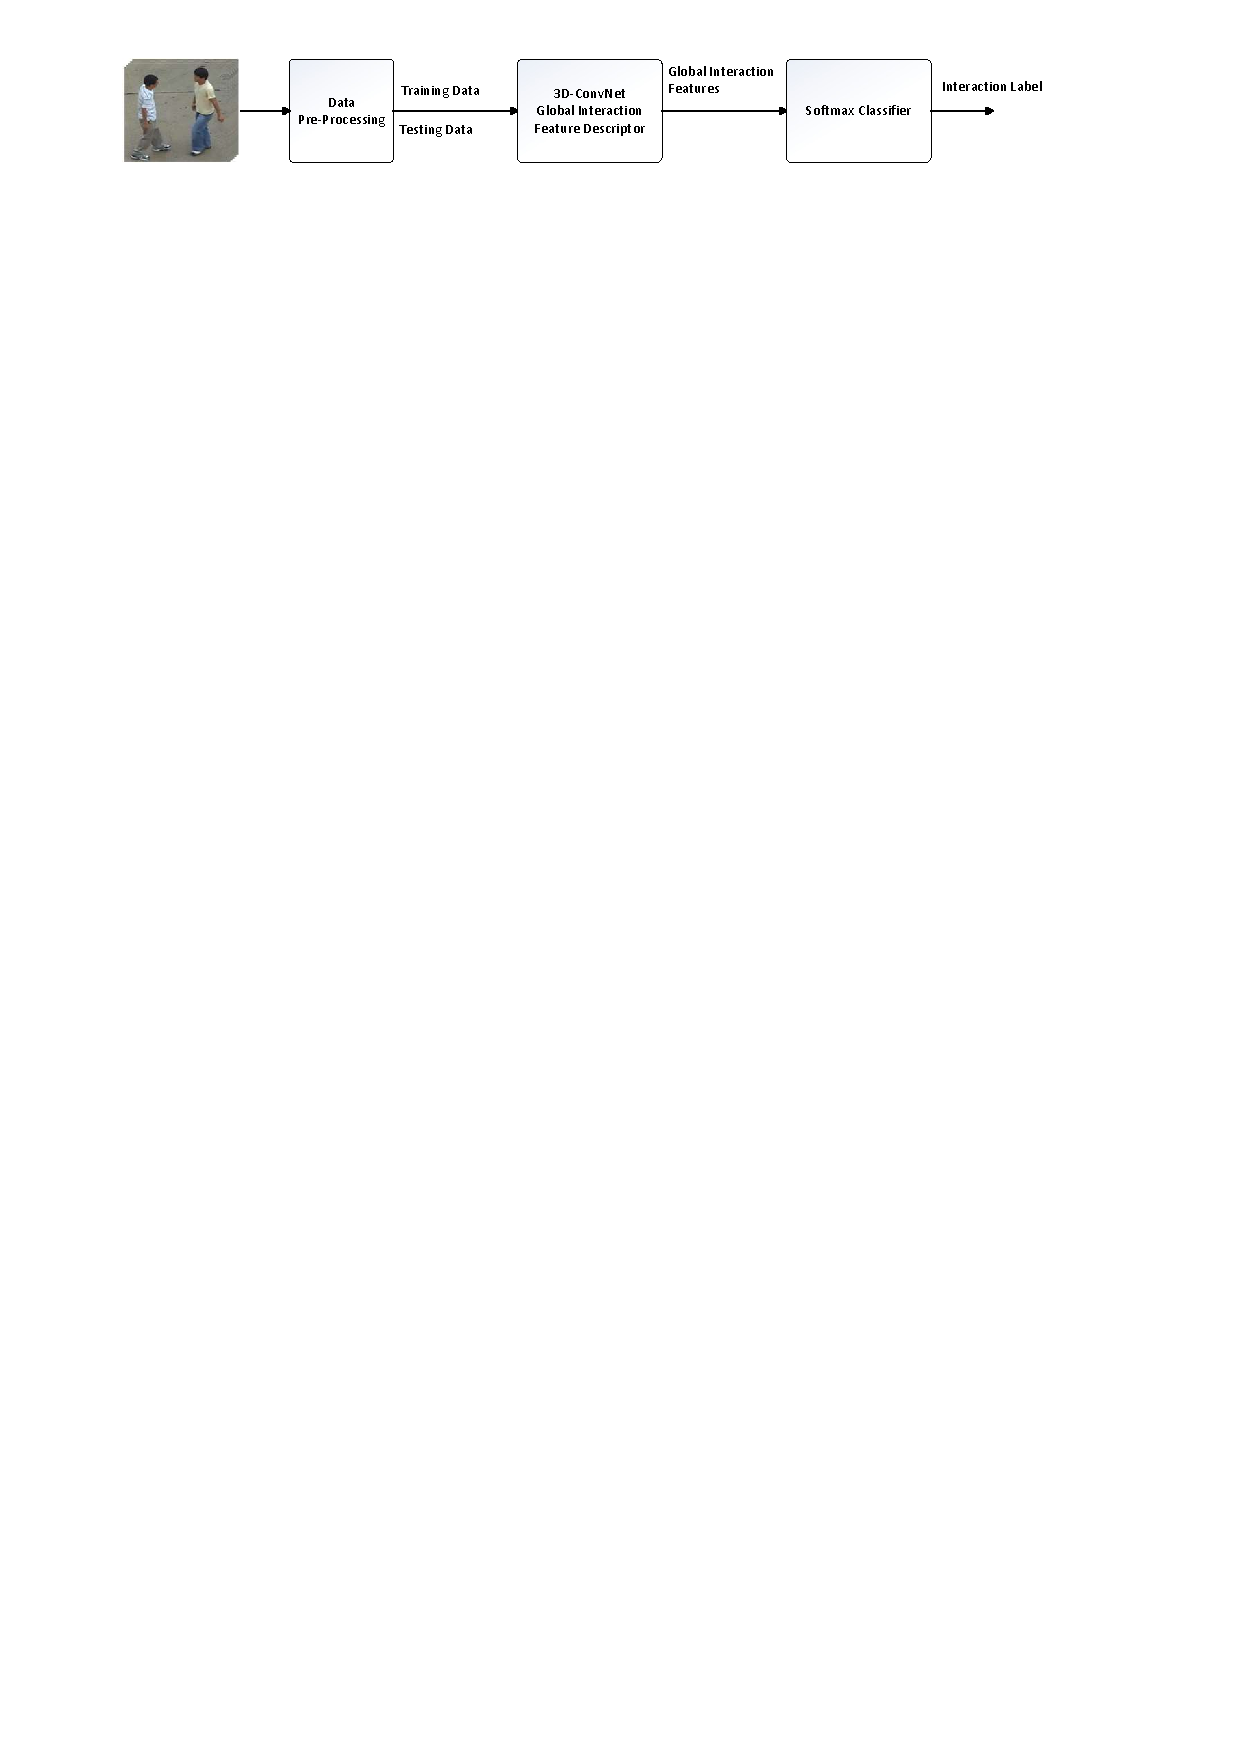
\includegraphics[trim=2cm 26.5cm 0cm 1cm]{fig01/arch_eval.pdf}
 	\caption{The architecture of the singleNet}
 	\label{fig:arch_eval}
 \end{figure}
Due to that we only need to search the optimal parameters by comparing the loss and classification accuracy between different parameter settings, it is not necessary to evaluate them on all data. For the sake of saving training time, it is reasonable to use part of the data instead of the all. So, all training and testing video used in the experiments of this section are from the UT-Interaction dataset set1, see Section \ref{ut-interaction}.  

\subsection{Assumptions and Factors and the default parameter setting}
Since there are many factors which influence the classification accuracy, and many parameters in each factor, it is impossible to search the optimal parameters by going through all the model parameters, at least under our current resource conditions. we test the effects of each parameter on the X as if they are independent. Based on this assumption, we have a set of default parameters as shown in Table \ref{table:default_paras}. We only adjust the parameters of one factor, keep the other parameters as default value, and observe the experimental results. At last, we use the combination of each factor's optimal parameter as our network's parameters and it is expected to be close to the optimal parameter combination.
  \renewcommand\arraystretch{1.2}  
  \begin{table}
  	\caption{Default parameters for network and data pre-processing}
  	\begin{center}
  		\begin{tabular}{| m{0.6cm} | m{7cm} | m{6cm} |}
  			\hline
  			\textbf{No.} & \textbf{Factors} & \textbf{Parameters}  \\ \hline \hline
  			% Network
  			\multicolumn{3}{|l|}{\textbf{Network}}  \\ \hline
  			
  			1 & Initial values of the network parameters, see Section \ref{Initialization}. & \tabincell{l} 
  						{\(weights = N(0,\sigma^2)\), \(\sigma = 0.01\) \\ 
  						 \(biases = 0.1 \)} \\ \hline
  			
  			2 & Dynamic adjusting of the learning rate, see Section \ref{learning_rate}. & \(Learning\ rate = 1e^{-4} \times 2^{-int(\frac{epoch}{4})} \)	\\ \hline
  			
  			3 & Dropout layers, see Section \ref{dropout} & \(keep\_ratio = 0.5\)	\\ \hline
  			
  			4 & Batch normalization layers, see Section \ref{bn} &  Yes  \\ \hline
  			
  			5 & The number of convolutional layers, see Section \ref{3dconv_layers} & 4\\ \hline
  			
  			6 & The size of convolutional kernels, see Section \ref{3dconv_filters} & \(3 \times 3 \times 3\) \\ \hline
  			
  			7 & The sizes of the pooling kernels, see Section \ref{3dconv_filters} & \tabincell{l}
  			                                       {L1: \(1 \times 2 \times 2 \) \\ 
  			                                       	L2, L3: \(2 \times 2 \times 2 \) \\
  				                                    L4: \(4 \times 2 \times 2 \)}   \\ \hline
  			                                    
  			8 &  The number of filters for each convolutional layer, see Section \ref{3dconv_filters} &  \tabincell{l}
  														{nof\_conv1 = 32 \\ 
  														nof\_conv2 = 128 \\
  														nof\_conv3 = 256 \\
  														nof\_conv4 = 512}   \\ \hline
  													
  			9 &  The number of output neurons for each fully connected layer, see Section \ref{fc} & \(\text{noo\_fc}_*\) = 4096 \\ \hline \hline                           
  			
  			% Network
  			\multicolumn{3}{|l|}{\textbf{Data pre-processing}}  \\ \hline
  			1 & Data augmentation: horizontal flipping, see Section \ref{pre_processing} \ref{augmentation} & Yes  \\ \hline
  			2 & Data augmentation: random cropping, see Section \ref{pre_processing} \ref{augmentation} & Yes, 4 times \\ \hline
  			3 & Temporal down-sampling of frames, see Section \ref{pre_processing} \ref{down-sampling} & Yes, N=0, see \ref{down-sampling} \\ \hline

  			4 & Data normalization, see Section \ref{pre_processing} \ref{normalization} & Yes, \(X_i = \frac{X_i - Mean(X)}{Std(X)}\) \\ \hline			
  		\end{tabular}
  		\label{table:default_paras}
  	\end{center}
  \end{table} 
   
\subsection{Experiments}
%***********************************************
% initializations
%**********************************************
\subsubsection{Initialization of the network parameters}
\paragraph{Experimental scheme}
To observe how much the initial values of the weights affect the classification accuracy,  we evaluated two initialization methods, including normal distribution with zero mean  and "Xavier" method \cite{xavier}. We evaluated the "Xavier" initialization with the uniform distribution to compare the performance between the two main-stream initialization schemes. We initialize all biases to \(0.1\) when we evaluate the weights initializations.
\par 
It's possible and common to initialize the biases to zero, but we only tested non-zero initial biases  because we use ReLU non-linearities and non-zero initialization of biases ensures that all ReLU units fire in the beginning and therefore obtain and propagate some gradient. We evaluated 3 constant value initializations for biases, including 0,001, 0.01 and 0.1. 

\paragraph{Experimental results and analysis}
 
The experimental results of comparison between "Xavier" and normal distribution initialization (\(\mu = 0, \sigma = 0.1\)) are illustrated in Figure \ref{fig:plot_xavier_vs_normal}.  The experimental results of the three different initial biases are illustrated in Figure \ref{fig:plot_biases}. 

\begin{figure}
	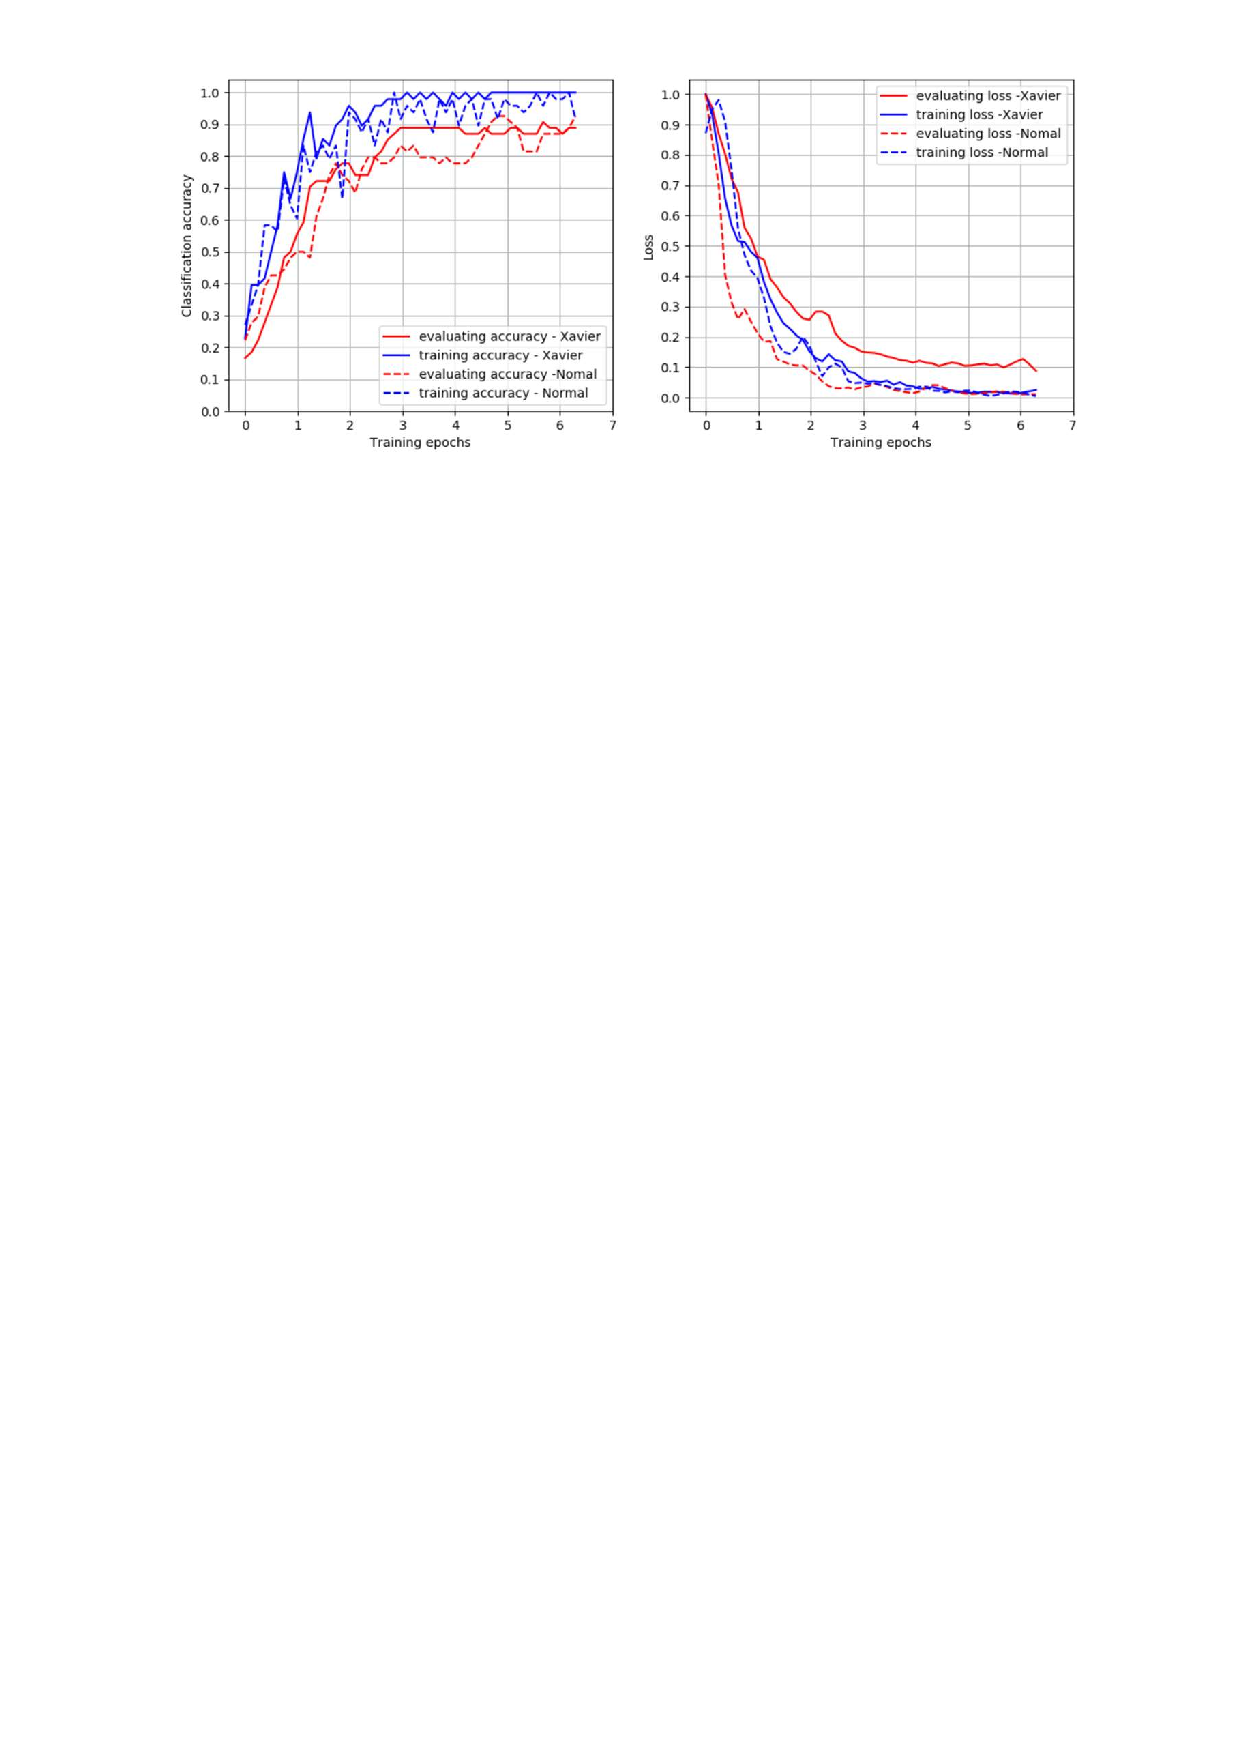
\includegraphics[trim=3cm 22cm 0cm 1cm]{fig01/plot_xavier_vs_normal.pdf}
	\caption{The loss and classification accuracy vs. training epochs comparison between "Xavier" and normal distribution initialization.}
	\label{fig:plot_xavier_vs_normal}
\end{figure}

 \begin{figure}
	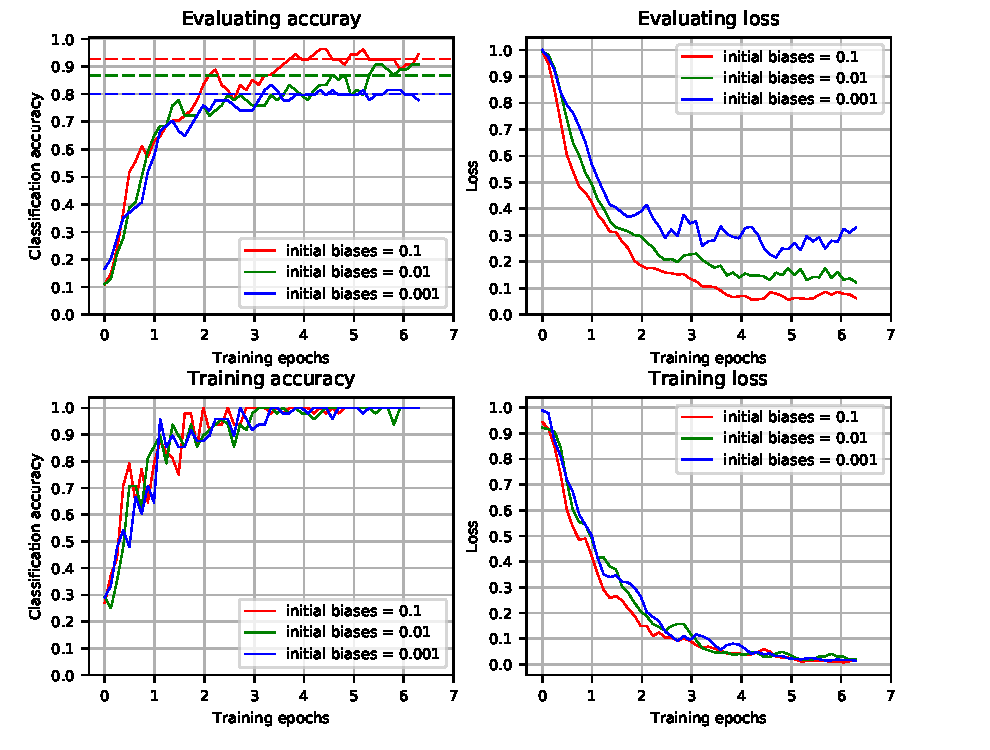
\includegraphics[trim=0cm 0cm 0cm 0cm]{fig01/plot_biases.pdf}
	\caption{The loss and classification accuracy vs. training epochs comparison between different initial biases.}
	\label{fig:plot_biases}
\end{figure}

From the experimental results, we can get the following conclusions about the initializations of network parameters (weights and biases): 
\begin{enumerate}
	\item Under the same network configurations, "Xavier" initialization gets more stable classification accuracy that the normal distribution initialization. 
	\item The evaluating loss of the "Xavier" initialization is slightly larger that that of the normal distribution initialization. But this may be caused by the far larger initial loss value of the normal distribution initialization. There is no obvious over-fitting for both initializations.
	\item For the initialization of biases, networks with relative larger initial biases can converge faster and achieve better classification accuracy with the ReLU non-linearity.
\end{enumerate} 
So, we will employ "Xavier" initialization in our network and set the initial biases to 0.1. 
%***********************************************
% learning rate
%***********************************************
\subsubsection{Learning Rate}
\paragraph{Experimental scheme}
We tested both constant learning rate and decaying learning rate over the period of the training process.  For constant learning rate, we tested values including 0.001, 0.0001 and 0.00001. We also tested the case that the learning rate is divided by 2 after every 3 epochs with initial value 0.0001.
 
\paragraph{Experimental results and analysis}
The experimental results of the loss and classification accuracy vs. training epochs comparison between networks with different learning rate are illustrated in Figure \ref{fig:plot_lr}.
 \begin{figure}
	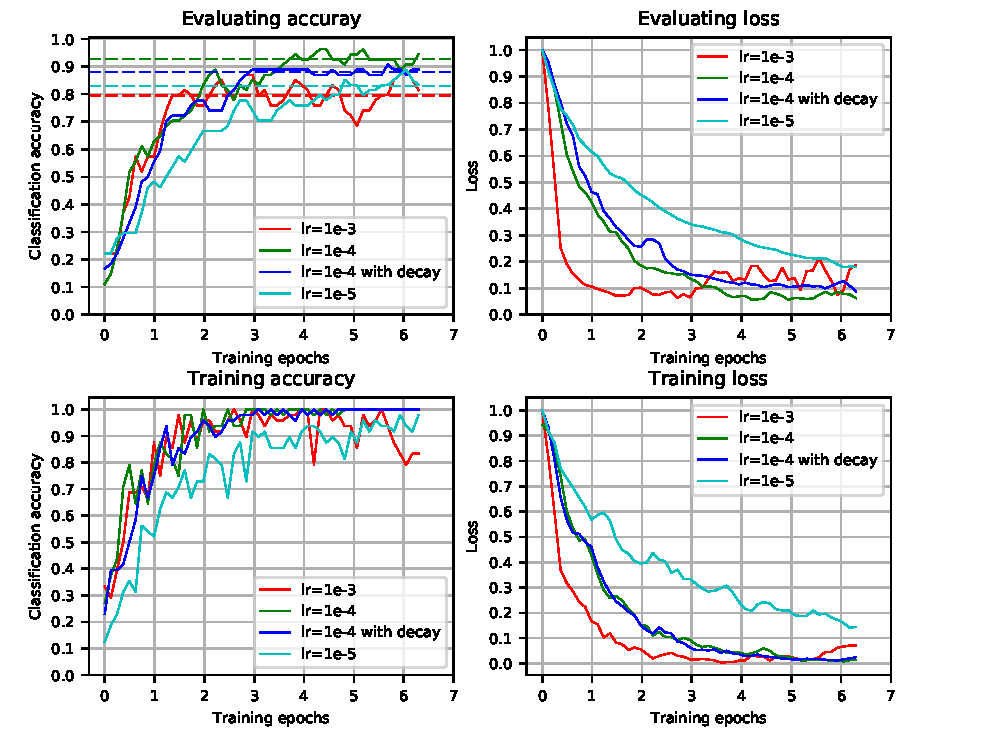
\includegraphics[trim=0cm 0cm 0cm 0cm]{fig01/plot_lr.pdf}
	\caption{The loss and classification accuracy vs. training epochs comparison between networks with different learning rate.}
	\label{fig:plot_lr}
\end{figure}
According to the experimental results, we can conclude the following for the learning rate:
\begin{enumerate}
	\item Larger learning rate, e.g. \(1e-3\), accelerates the convergence speed of the network, but it is also easier to over-fit to the training data and even causes unstability.
	\item The training process with smaller learning rate, e.g. \(1e-5\), converges slowly. 
	\item The training processes with learning rate \(1e-4\) has good balance between the performance and convergency speed. And whether decay the learning rate over to the training epochs doesn't affect much of the performance.   
\end{enumerate}
So, we set the learning rate to \(1e-4\) for our network.

%***********************************************
% dropout
%***********************************************
\subsubsection{Dropout layer}
\paragraph{Experimental scheme}
Dropout layer is considered as an extremely effective way to reduce over-fitting in neural network,see Section \ref{fc}. We tested different values of the probability \(p\), including 0.8, 0.5, 0.2.

\paragraph{Experimental results and analysis}
The experimental results of the loss and classification accuracy vs. training epochs comparison between different keep probabilities of the dropout layers are illustrated in Figure \ref{fig:plot_dropout}.
\begin{figure}
	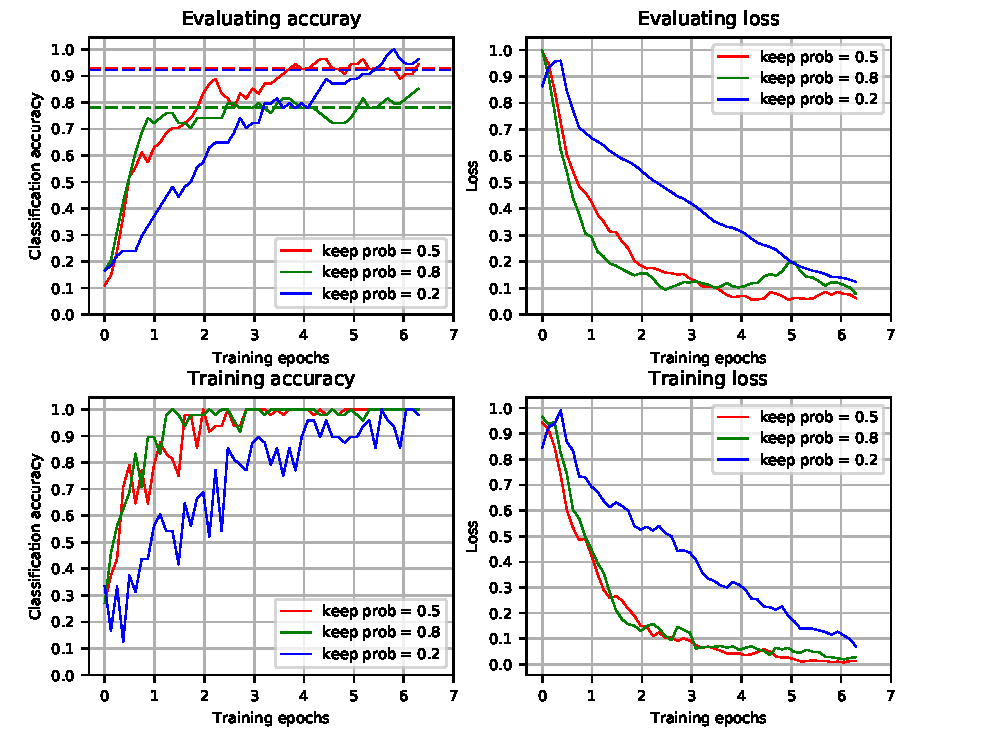
\includegraphics[trim=0cm 0cm 0cm 0cm]{fig01/plot_dropout.pdf}
	\caption{The loss and classification accuracy vs. training epochs comparison between different keep probabilities in the dropout layers.}
	\label{fig:plot_dropout}
\end{figure}

According to the experimental results, we conclude the following for the keep probabilities in the dropout layers:
\begin{enumerate}
	\item Larger keep probability (0.8) in the dropout layers makes the network converge faster, but the classification accuracy remains at a lower level after convergence.
	\item Smaller keep probability (0.2) in the dropout layers makes the network converge slower, but the final classification accuracy is higher after convergence.
	\item 0.5 is a reasonable value of keep probability because it has a good balance between performance and convergence speed.
\end{enumerate}
So, we set the keep probabilities to 0.5 in our network. 

%***********************************************
% batch normalization
%***********************************************
\subsubsection{Batch normalization layer}
\paragraph{Experimental scheme}
To observe the effects of batch normalization (BN) layers, see Section \ref{bn}, we compared the loss and classification accuracy between the network with and without BN layers. The only difference between the two networks is whether there are BN layers after the first two ReLU layers.  

\paragraph{Experimental results and analysis}
The experimental results of the loss and classification accuracy vs. training epochs comparison between networks with and without BN layers are illustrated in Figure \ref{fig:plot_bn_en}.
 \begin{figure}
	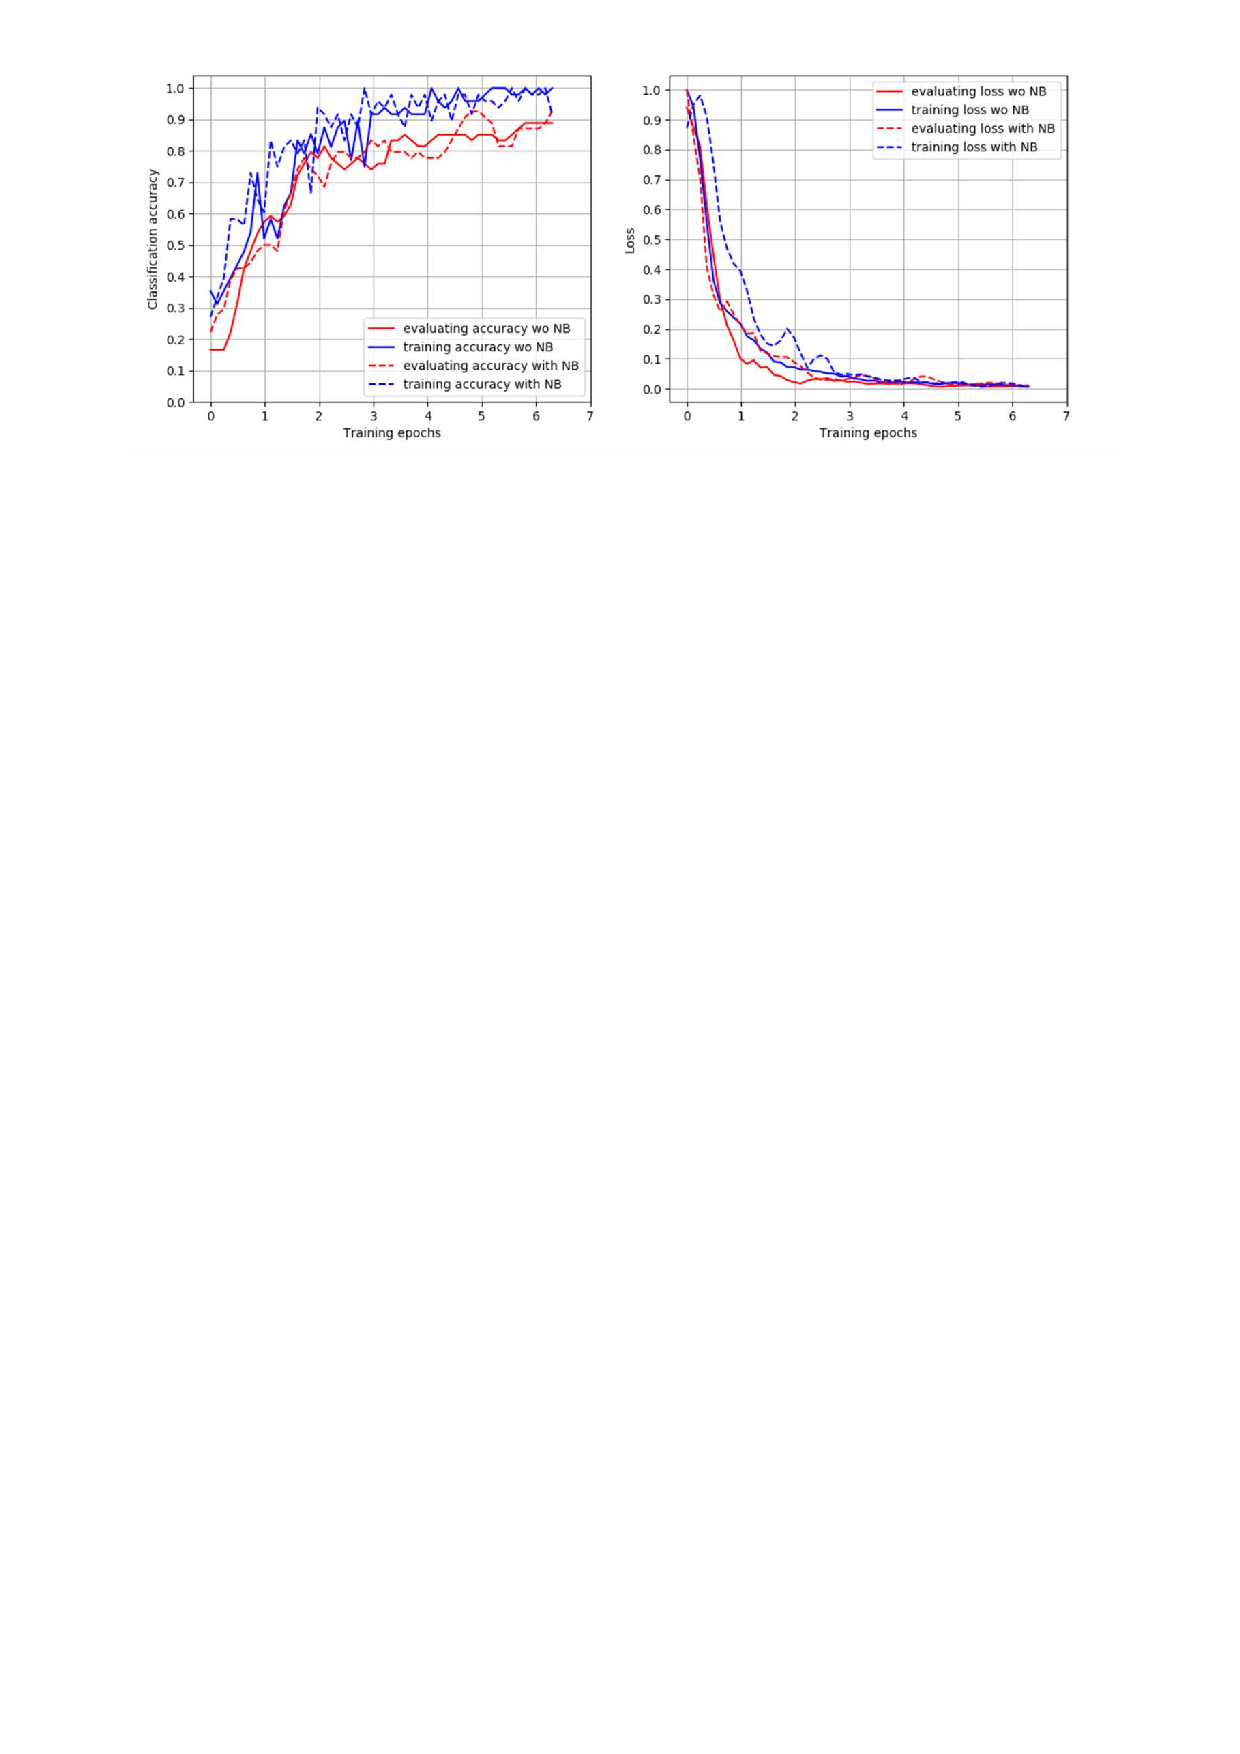
\includegraphics[trim=2.5cm 22.5cm 0cm 1cm]{fig01/plot_bn_en.pdf}
	\caption{The loss and classification accuracy vs. training epochs comparison between networks with and without batch normalization layers.}
	\label{fig:plot_bn_en}
\end{figure}

According to the experimental results, we can say about the  batch normalization layers: 
\begin{enumerate}
	\item The convergence speed between the network with and without BN layers is similar.
	\item The network with batch normalization layers gets slightly higher classification accuracy, about 0.92, than the network without batch normalization layers, about 0.88.
\end{enumerate}
So, we add batch normalization layers in our network. 

%***********************************************
% the number of convolution layers
%***********************************************
\subsubsection{The number of the convolutional layers}
\paragraph{Experimental scheme}
Generally, the network can get stronger global information representing ability and nicer non-linearity by applying multiple convolutional layers. In our project, we tested 3 networks with different numbers of 3D convolutional layers: 4, 5 and 6, respectively. The structures and parameters of the three networks are illustrated in Figure \ref{fig:cnn_layers}.
\begin{figure}
 	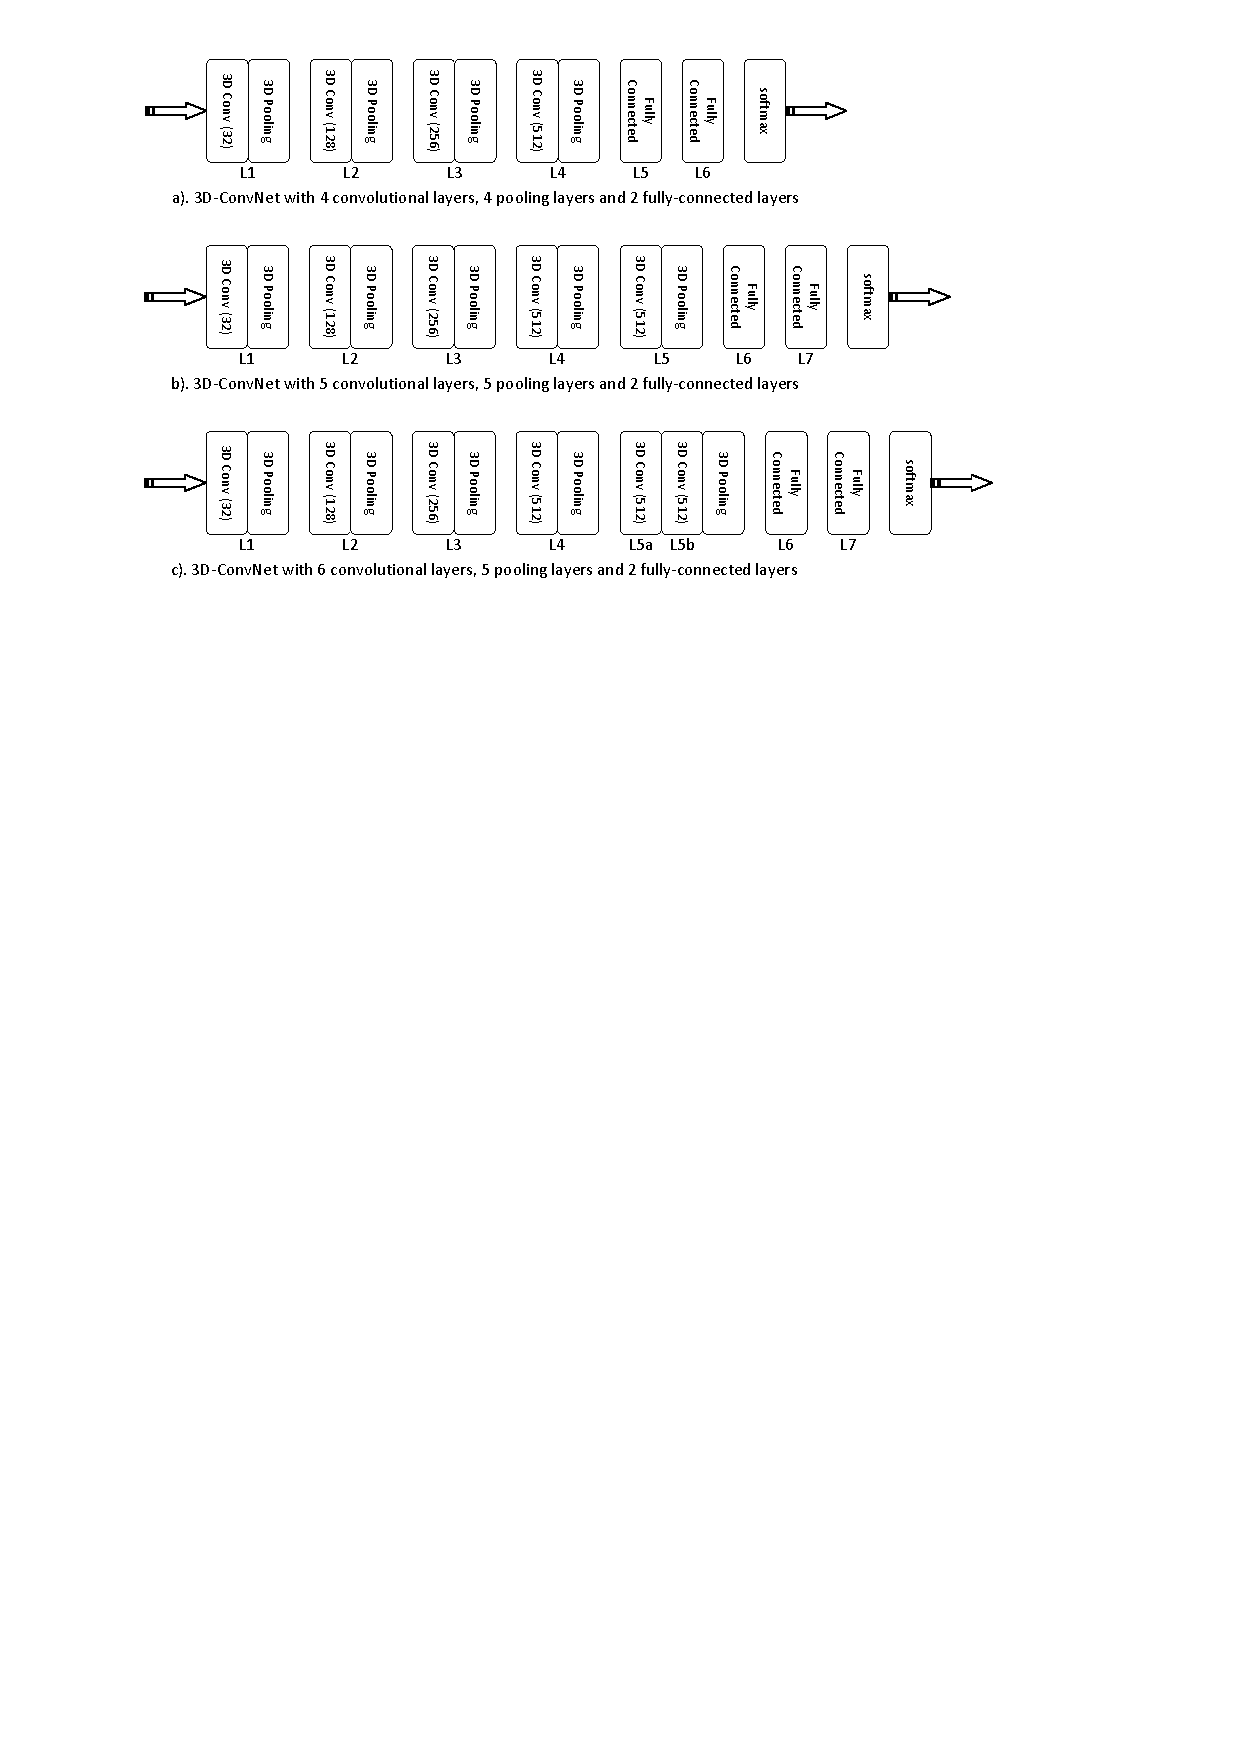
\includegraphics[trim=1cm 20cm 0cm 1cm]{fig01/cnn_layers.pdf}
 	\caption{The structures and parameters of the three 3DConvNets which have different number of convolutional layers.}
 	\label{fig:cnn_layers}
\end{figure}
\paragraph{Experimental results and analysis}
According to the experimental results, as shown in Figure \ref{fig:plot_layers}, we can get following conclusions about the different number of the 3D convolutional layers: 
\begin{enumerate}
	\item The convergence speed is not affected by the number of the 3D convolutional layers.
	\item The 3DConvNet with 5 convolutional layers gets the best classification accuracy among the three. This may because that the more layers the stronger global information representing ability. But at the same time, the network with more layers also needs to be trained on richer training data, else, it may perform even worse, e.g. the case of the 3DConvNet with 6 convolutional layers.
\end{enumerate}
\begin{figure}
	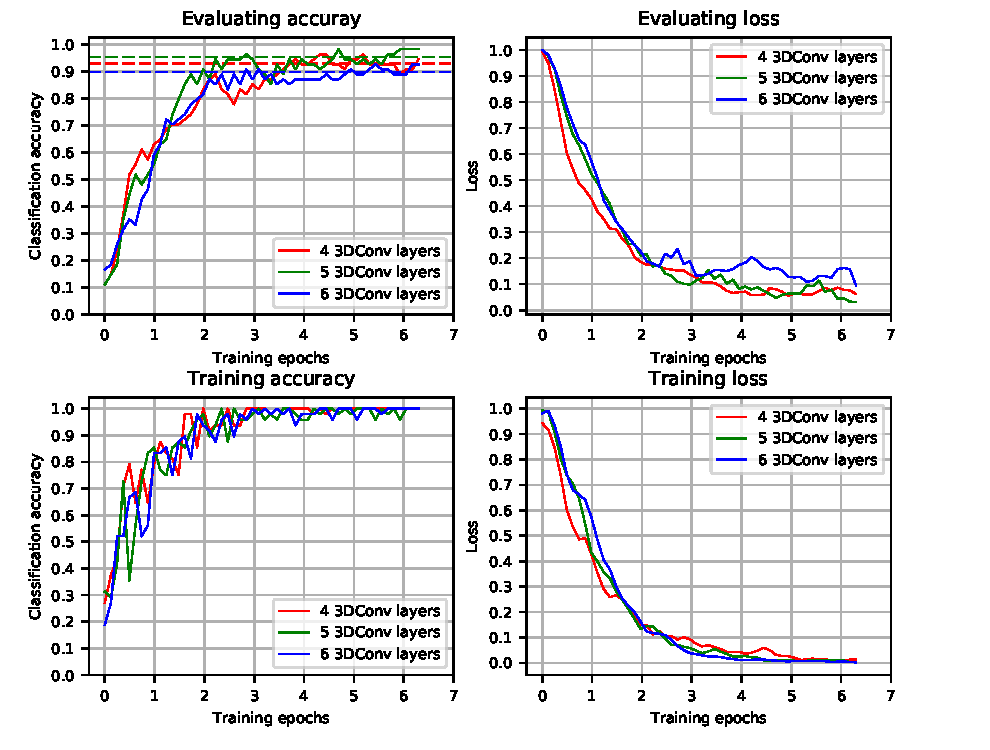
\includegraphics[trim=0cm 0cm 0cm 1cm]{fig01/plot_layers.pdf}
	\caption{The loss and classification accuracy vs. training epochs comparison between networks with different convolutional layers.}
	\label{fig:plot_layers}
\end{figure}

So, we set 5 convolutional layers in our 3DConvNet.


%***********************************************
% the size of the convolutional kernel
%***********************************************
\subsubsection{The size of the convolutional kernel}
\paragraph{Experimental scheme}
We evaluate how much the performance relates to the size of convolutional kernels by comparing four networks with different convolutional kernel sizes: \(3 \times 3 \times 3\), \(3\times 4 \times 4\), \(4\times4\times4\) and \(4\times 4 \times 3\), see Section \ref{3dconv_filters} for the format of kernel size. We set all convolutional layers to use the same kernel size in each 3DConvNet. 

\paragraph{Experimental results and analysis}
According to the experimental results, as shown in Figure \ref{fig:plot_cnn_kernel}, we found that there is no obvious difference both in the convergence speed and classification accuracy among the networks with different convolutional kernel sizes. So, we keep using the size of \(3\times 3 \times 3\) for all convolutional kernels.
\begin{figure}
	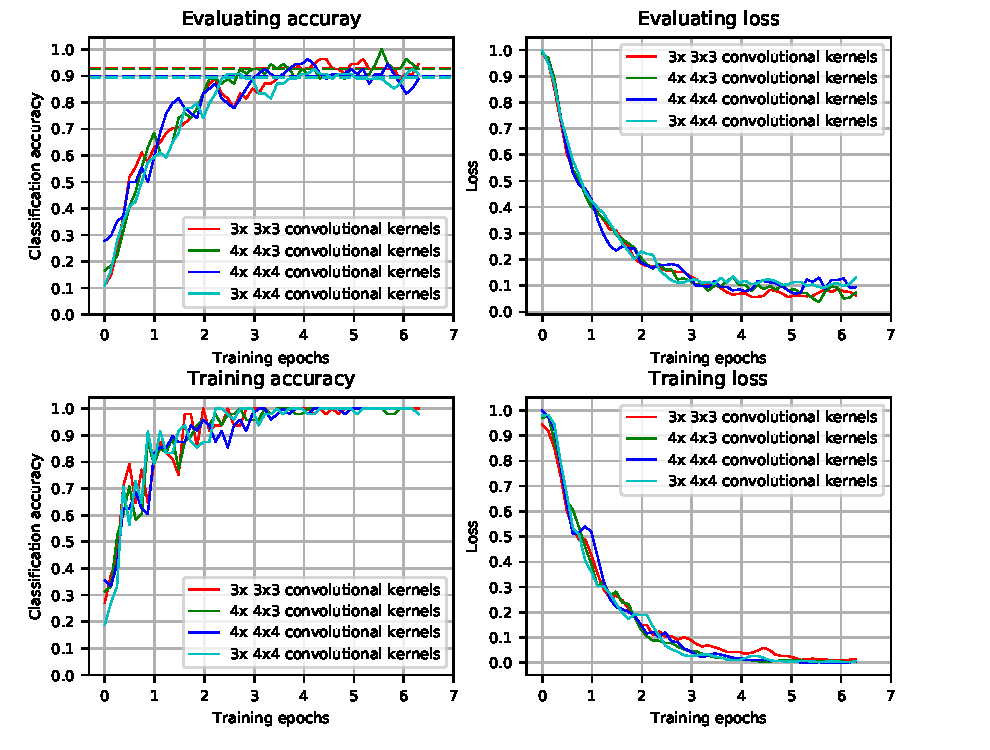
\includegraphics[trim=0cm 0cm 0cm 0cm]{fig01/plot_cnn_kernel.pdf}
	\caption{The loss and classification accuracy vs. training epochs comparison between networks with different sizes of the convolutional kernels.}
	\label{fig:plot_cnn_kernel}
\end{figure}


%***********************************************
% The number of filters for each convolutional layer
%***********************************************
\subsubsection{The number of filters of each convolutional layer}
\paragraph{Experimental scheme}
We use a 3DConvNet with 4 convolutional layers to evaluate the relationship between the performance and the number of filters of each convolutional layer. We performed four experiments which adjust the number of filters for only one convolutional layer each time, including 1) \(nof\_conv1\ 32 \rightarrow 64\), 2) \(nof\_conv2\ 128 \rightarrow 64\), 3) \(nof\_conv3\ 256 \rightarrow 512\), and 4) \(nof\_conv4\ 512 \rightarrow 256\).

\paragraph{Experimental results and analysis}
The experimental results are illustrated in Figure \ref{fig:plot_nof}. The numbers listed in the legend represent the numbers of the filters for each convolutional layer, e.g. \([32,128,256,512]\) represents \(nof\_conv1 = 32, nof\_conv2 = 128, nof\_conv3 = 256, nof\_conv4 = 512\). 
\par 
According to the experimental results, the networks perform a little better when the numbers of the filters are  \([32,128,256,512]\) and \([32,128,512,512]\), while the performance is a little worse when the numbers of the filters are \([32,64,256,512]\).
It is hard to explain why they perform better or worse from the limited experimental data. We just use  \([32,128,256,512]\) to configure the convolutional layers of our network.  
\begin{figure}
	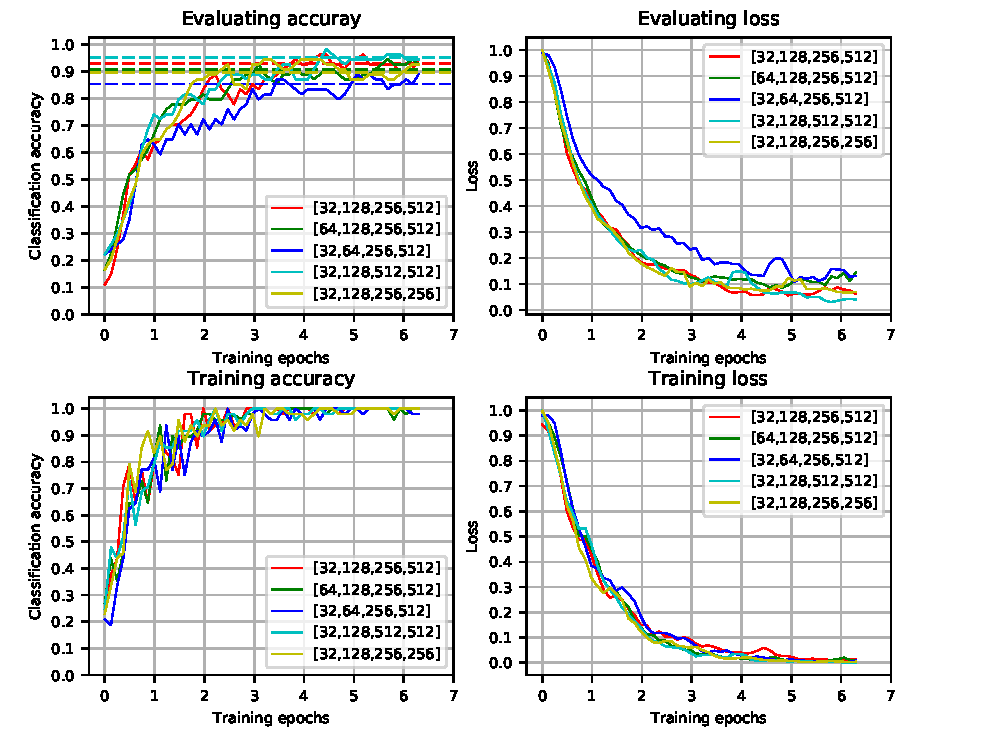
\includegraphics[trim=0cm 0cm 0cm 0cm]{fig01/plot_nof.pdf}
	\caption{The loss and classification accuracy vs. training epochs comparison between networks with different number of filters in each convolutional layer.}
	\label{fig:plot_nof}
\end{figure}



%***********************************************
% The number of neurons for each fc layer
%***********************************************
\subsubsection{The number of neurons of each fully connected layer}
\paragraph{Experimental scheme}
There are two fully connected layers in our network. In this experiment, we compared the networks with different numbers of output neurons in the fully connected layers. Specifically, we compared three cases, including \([2048,2048]\), \([4096,2048]\) and \([4096,4096]\), where the numbers in the square bracket represent the number of output neurons of the fully connected layers, e.g. \([2048,2048]\) represents \(noo\_fc6 = 2048, noo\_fc7 = 2048\), where \(noo\_fc6\) is the notation of the number of output neurons of the FC6 layer.

\paragraph{Experimental results and analysis}
The experimental results are shown in Figure \ref{fig:plot_noo}. According to the experimental results, we conclude:
\begin{enumerate}
	\item The network converges a little faster with \([4096,4096]\) output neurons, while there is no obvious difference between \([2048,2048]\) and \([4096,2048]\).
	\item The network with \([4096,4096]\) output neurons also performs a little better than the networks with  \([2048,2048]\) and \([4096,2048]\) output neurons. 
\end{enumerate}
So, we  use  \([4096,4096]\) to configure the fully connected layers of the network.
 
\begin{figure}
	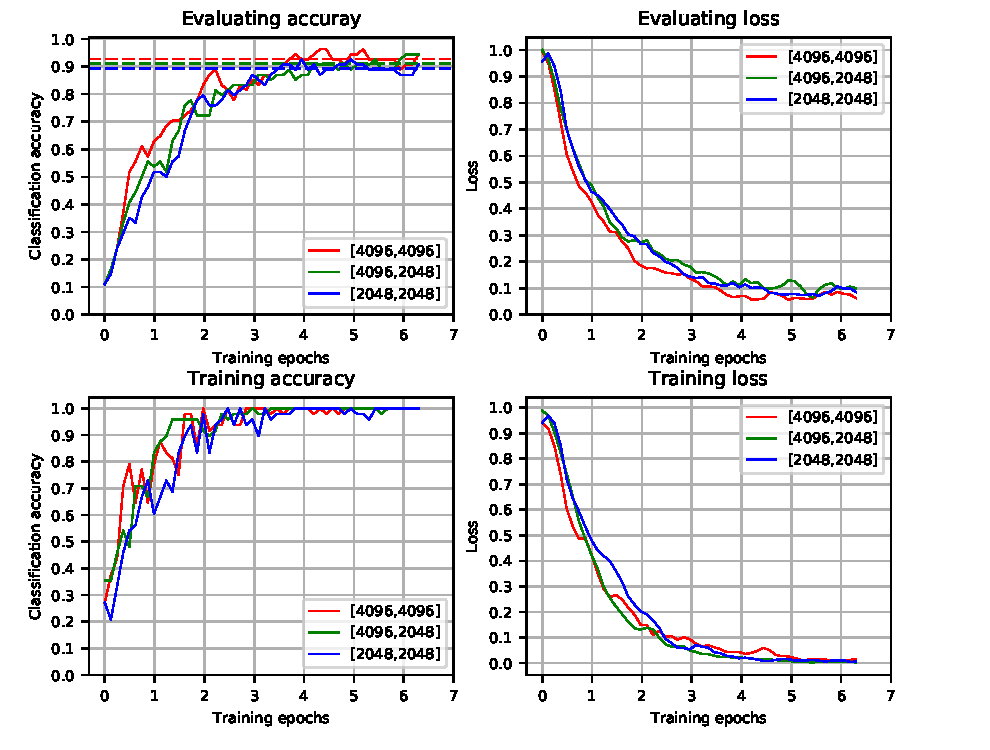
\includegraphics[trim=0cm 0cm 0cm 0cm]{fig01/plot_noo.pdf}
	\caption{The loss and classification accuracy vs. training epochs comparison between networks with different number of output neurons in each fully connected layer.}
	\label{fig:plot_noo}
\end{figure}


%***********************************************
% Data augmentation: horizontal flipping
%***********************************************
\subsubsection{Data augmentation: horizontal flipping}
\paragraph{Experimental scheme}
Horizontal flipping is a common technique to augment the training data, especially for the small scale training data, see Section \ref{pre_processing} \ref{augmentation}. We evaluated two networks trained on the data with and without horizontal flipping. 

\paragraph{Experimental results and analysis}
According to the experimental results, shown in Figure \ref{fig:plot_rlf}, the network trained on the data with horizontal flipping significantly outperforms the network which is trained on the data without horizontal flipping. So, we adopt the horizontal flipping technique to augment our training data. 
\begin{figure}
	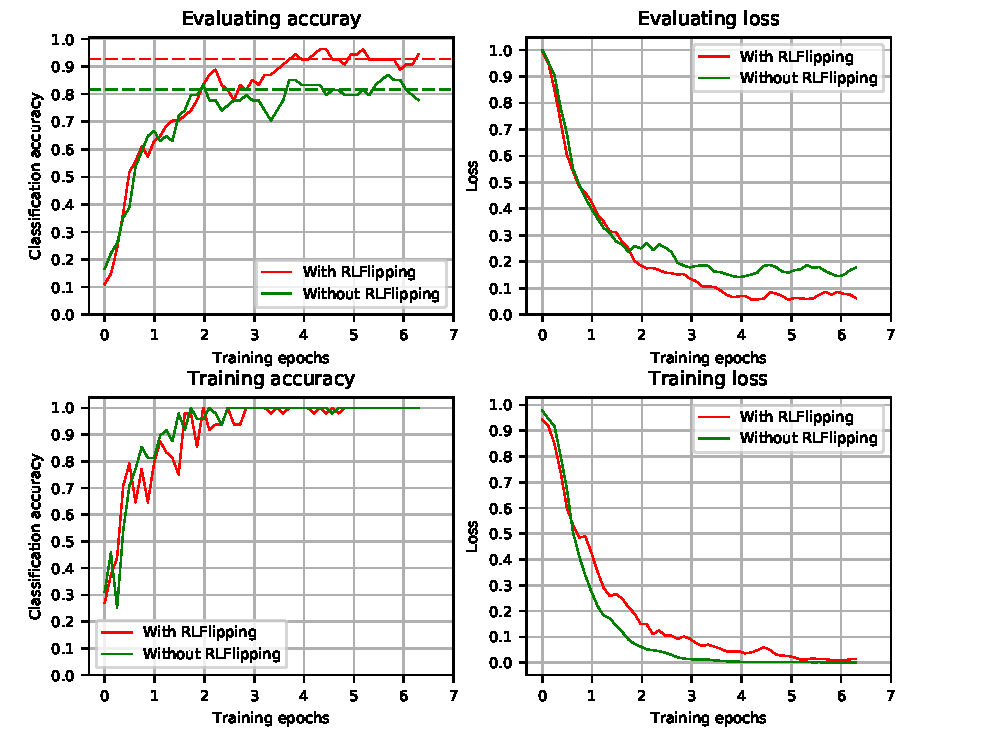
\includegraphics[trim=0cm 0cm 0cm 0cm]{fig01/plot_rlf.pdf}
	\caption{The loss and classification accuracy vs. training epochs comparison between networks trained on the data with and without horizontal flipping.}
	\label{fig:plot_rlf}
\end{figure}


%***********************************************
% Data augmentation: random cropping
%***********************************************
\subsubsection{Data augmentation: random cropping}
\paragraph{Experimental scheme}
N-time random cropping is another commonly used technique to augment small scale training data, see Section \ref{pre_processing} \ref{augmentation}. We evaluated three networks trained on the data with 3 different random cropping configurations, including 1-time random cropping, 2-time random cropping, and 4-time random cropping. 

\paragraph{Experimental results and analysis}
The experimental results are illustrated in Figure \ref{fig:plot_rc}. According to the experimental results, the random cropping technique does help a lot in training the network. The network trained on the data with 4-time random cropping outperforms that with 2-time random cropping, and the network trained on the data with 2-time random cropping outperforms that with 1-time random cropping. So, we use the 4-time random cropping to augment our training data in the project.
\begin{figure}
	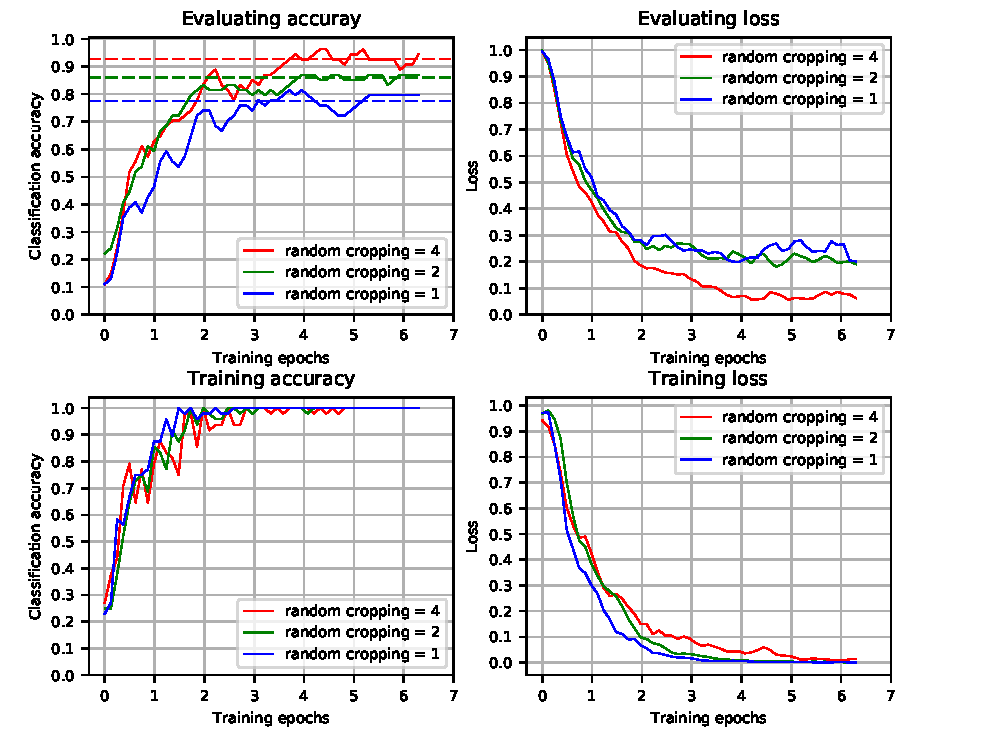
\includegraphics[trim=0cm 0cm 0cm 0cm]{fig01/plot_rc.pdf}
	\caption{The loss and classification accuracy vs. training epochs comparison between networks trained on training data with different random cropping configurations.}
	\label{fig:plot_rc}
\end{figure}


%***********************************************
% Temporal down-sampling of frames
%***********************************************
\subsubsection{Temporal down-sampling of frames}
\paragraph{Experimental scheme}
Temporal down-sampling of frames is a method which we applied to make each video clip contains more temporal information, see Section \ref{pre_processing} \ref{down-sampling}. We evaluated 4 cases: including temporal down-sampling with temporal strides 1 frame, 2 frames, 3 frames and evenly sample 16 frames from each video (temporal down-sampling = 0).  

\paragraph{Experimental results and  analysis}
The experimental results are illustrated in Figure \ref{fig:plot_tds}. The network trained on the data which are evenly sampled 16 frames from each input video performs the best. And the other three network have similar performance. So, we set the temporal down-sampling mode to 0 to pre-process our training data.
\begin{figure}
	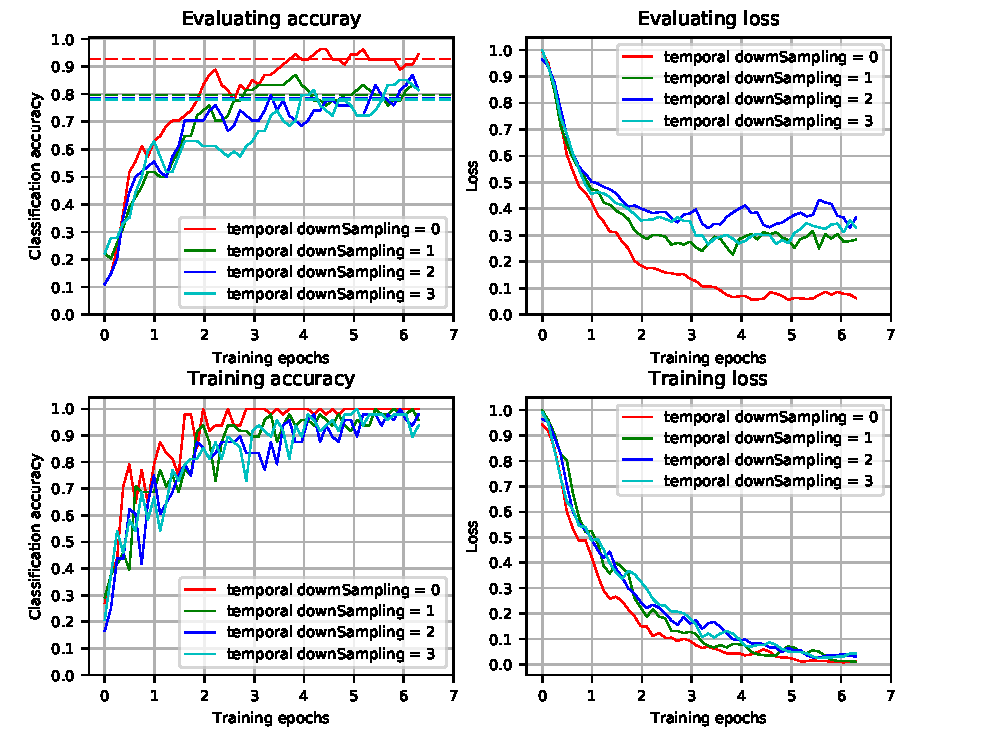
\includegraphics[trim=0cm 0cm 0cm 0cm]{fig01/plot_tds.pdf}
	\caption{The loss and classification accuracy vs. training epochs comparison between networks trained on training data with different temporal down-sampling strides.}
	\label{fig:plot_tds}
\end{figure}


%***********************************************
% Data normalization
%***********************************************
\subsubsection{Data normalization}
\paragraph{Experimental scheme}
Normalizing the data before feeding to the network is a common method, see Section \ref{pre_processing} \ref{normalization}. In this experiment, we evaluated three different data normalization methods, including: 1) directly scale the value of \(X\) from \(0-255\) to \(0-1\), 2) subtract the \(mean\) value (\(X-mean\)),  3) subtract the mean value and divide it by the standard deviation (\((X-mean)/std\)).   
\paragraph{Experimental results and analysis}
The experimental results are illustrated in Figure \ref{fig:plot_dnm}. According to the experimental results, the network trained on the data with normalization mode (\(X -mean\)) performs best among the three, and the other two networks have similar performance. So, we use the normalization mode (\(X -mean\)) to normalize the data in our project.
\begin{figure}
	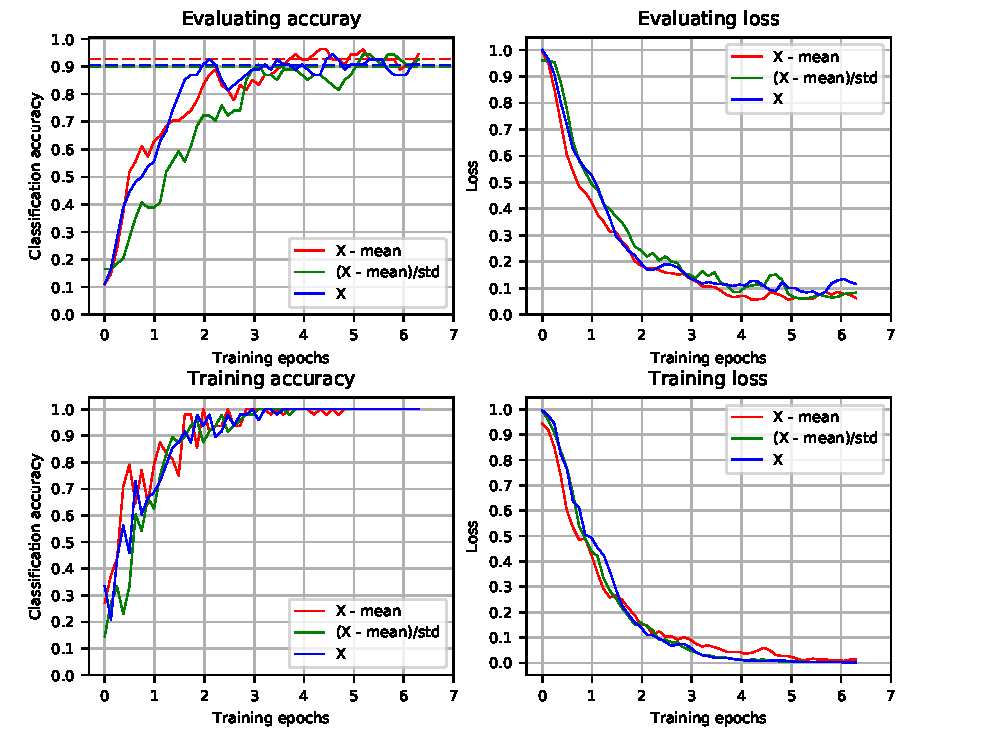
\includegraphics[trim=0cm 0cm 0cm 0cm]{fig01/plot_dnm.pdf}
	\caption{The loss and classification accuracy vs. training epochs comparison between networks trained on training data with different normalization methods.}
	\label{fig:plot_dnm}
\end{figure}

\subsection{Conclusions of parameter searching}
According to all of the above experiments which we performed for parameter searching, we can obtain following conclusions:
\begin{enumerate}
	\item In the network side,  the factors which affect the performance much are not the hyper-parameters of the network but those factors in the training processing, including the initialization of network parameters, learning rate and the keep probability of the dropout layers. 
	\item In the data pre-processing side, almost all factors except the data normalization method affect the performance of the network much.  Such conclusion also indicates that the data is the critical factor of our project.   
\end{enumerate}

\section{The experimental results of of the interaction classification}
\subsection{Train the network from scratch}
\subsubsection*{Experimental scheme}
In this step, we train the fullNet on UT-Interaction dataset from scratch. We face a new problem when we try to apply all optimal parameter settings from singleNet to fullNet. That is the overall GPU memory allocation requirement for the fullNet is larger than 24GiB which is beyond the GPU resource we have in hand. So, we slightly adjust the hyper-parameters of the fullNet. The adjusted hyper-parameters are the values of \(noo\_fc5\) and \(noo\_fc6\) , and both from \(4096\) to \(2048\). To compare the performance between the fullNet and singleNet, we build three models: a). fullNet with adjusted hyper-parameters notated as fullNet\_2048, b). singleNet with optimal hyper-parameters notated as singleNet\_4096, and c). singleNet with adjusted hyper-parameters notated as singleNet\_2048.  The data pre-processing methods and parameter settings, the architecture and hyper-parameter settings of the network, and the training settings are illustrated in the Table \ref{table:network_settings}.
  
  \renewcommand\arraystretch{1.2}  
\begin{table}
	\caption{Parameter, network architecture and training settings for network and data pre-processing.}
	\begin{center}
		\begin{tabular}{| m{0.6cm} | m{7cm} | m{6cm} |}
			\hline
			\textbf{No.} & \textbf{Factors} & \textbf{Parameters}  \\ \hline \hline
			% Network
			\multicolumn{3}{|l|}{\textbf{Network}}  \\ \hline
			
			1 & Initial values of the network parameters, see Section \ref{Initialization}. & \tabincell{l} 
			{ \(weights\) : "Xavier" initialization \\ 
				\(biases\) : constant 0.1} \\ \hline
			
			2 & Dynamic adjusting of the learning rate, see Section \ref{learning_rate}. & \(Learning\ rate = 1e^{-4} \)	\\ \hline
			
			3 & Dropout layers, see Section \ref{dropout} & \(keep\_ratio = 0.5\)	\\ \hline
			
			4 & Batch normalization layers, see Section \ref{bn} &  Yes  \\ \hline
			
			5 & The number of convolutional layers, see Section \ref{3dconv_layers} & 5\\ \hline
			
			6 & The size of convolutional kernels, see Section \ref{3dconv_filters} & \(3 \times 3 \times 3\) \\ \hline
			
			7 & The sizes of the pooling kernels, see Section \ref{3dconv_filters} & \tabincell{l}
			{L1: \(1 \times 2 \times 2 \) \\ 
				L2, L3, L4: \(2 \times 2 \times 2 \) \\
				L5: \(2 \times 1 \times 1 \)}   \\ \hline
			
			8 &  The number of filters for each convolutional layer, see Section \ref{3dconv_filters} &  \tabincell{l}
			{nof\_conv1 = 32 \\ 
			nof\_conv2 = 128  \\
			nof\_conv3 = 256  \\
			nof\_conv4 = 512 \\
			nof\_conv5 = 512}  \\ \hline
			
			9 &  The number of output neurons for each fully connected layer, see Section \ref{fc} & \(\text{noo\_fc}_*\) = 4096 \\ \hline \hline                           
			
			% Network
			\multicolumn{3}{|l|}{\textbf{Data pre-processing}}  \\ \hline
			1 & Data augmentation: horizontal flipping, see Section \ref{pre_processing} \ref{augmentation} & Yes  \\ \hline
			2 & Data augmentation: random cropping, see Section \ref{pre_processing} \ref{augmentation} & Yes, 4 times \\ \hline
			3 & Temporal down-sampling of frames, see Section \ref{pre_processing} \ref{down-sampling} & Yes, N=0, see \ref{down-sampling} \\ \hline
			
			4 & Data normalization, see Section \ref{pre_processing} \ref{normalization} & Yes, \(X_i = X_i - Mean(X)\) \\ \hline			
		\end{tabular}
		\label{table:network_settings}
	\end{center}
\end{table} 
\subsubsection*{Experimental results}
The classification accuracy comparisons among different models are illustrated in Table \ref{table:threeModels}.  The classification accuracy of the \(singleNet\_4096\) is slightly better than that of the \(fullNet\_2048\). But this doesn't mean that the \(singleNet\) always performances better than that of the \(fullNet\), because the \(singleNet\_2048\) only gets \(82.4\%\) classification accuracy. So, the performance of the \(fullNet\_4096\) is expected to achieve better performance than the \(fullNet\_2048\) according to the comparison between the \(singleNet\_4096\) and the \(singleNet\_2048\), but we don't have enough GPU memory resource to run the model. The classification accuracy of our model are not as good as the works of Raptis et al. \cite{raptis} and Zhang et al. \cite{yimeng}. One possible reason is that both the above two works take body parts into consideration, so, they can focus on these discriminative parts and thus get higher performance. While, in our method, we use deep learning method to learn features from the whole video not from some specific body parts.  

\begin{table}
	\caption{The performance comparisons among different models, evaluated on UT-Interaction set1.}
	\begin{center}
		\begin{tabular}{| m{4cm} | m{4cm} |}
			\hline
			Model & Classification Accuracy \\ \hline \hline
			our fullNet\_2048 & 87.4\%   \\ \hline
			our singleNet\_4096 & 88.8\% \\ \hline
			our singleNet\_2048 & 82.4\%  \\ \hline
			Raptis\&Sigal \cite{raptis} & 93.3\%        \\ \hline
			Zhang et al. \cite{yimeng} & 90\%  \\ \hline
			Ryoo \cite{ryoo2011}  & 85\% \\ \hline
			 				
		\end{tabular}
		\label{table:threeModels}
	\end{center}
\end{table}


\section{The experimental results of of the interaction detection}
The goal of interaction detection in UT-Interaction is to locate interactions spatially and temporally in a given un-segmented video which contains approximately 6 interactions in each single video. Since the performance of the interaction detection is highly dependent on the quality of  the interacting people detection, we first present the results of the interacting people detection, then the details of the performance of the interaction detection.    

\subsection{Results of the interacting people detection} 
\subsubsection*{Experimental scheme}
We use the overlap ratio between the detected bounding boxes of the interacting people and the bounding boxes of the ground truth to measure the quality of the interacting people detection for each video. The detailed method includes: 
\begin{enumerate}
	\item Detect the interacting people at each frame.
	\item Calculate the overlap ratio of the bounding boxes between the detected one and the one from the ground truth with the following formula:
	\begin{equation}
		overlap\ ratio = \frac{\text{Detection} \cap \text{Ground Truth}}{\text{Detection} \cup \text{Ground Truth}}
	\end{equation}
	\item Average the overlap ratios over all frames which are annotated containing interactions by the ground truth:
	\begin{equation}
		mean \ overlap\ ratio = \frac{1}{M}\sum_{i=1}^{M} overlap\ ratio
	\end{equation}
\end{enumerate} 
\subsubsection*{Experimental results}
The detailed mean spatial overlap ratios for all videos of the UT-Interaction dataset set1 are illustrated in Table \ref{table:mean_overlap_ratio}. And the qualitative experimental results are illustrated in Figure \ref{fig:int_det} with interacting people bounding boxes annotated for set1, the red one is the detection and the green one is the ground truth. The interacting people detections for the sequences 1 to 4 are easy since there are only two interacting people appear in the scene, but it is more challenging to locate the positions of interacting people for sequences 5 to 10, because both interacting people and irrelevant pedestrians are present in the scene. We adopt the method mentioned in Chapter \ref{locate_interacting_people} to exclude the irrelevant people. From the experimental results shown in Figure \ref{fig:int_det}, we successfully locate the spatial positions of interacting people for all videos except sequence 9, because the relative position between the irrelevant people are very close to the target interacting people and they execute the activities simultaneously. 
\begin{figure}
	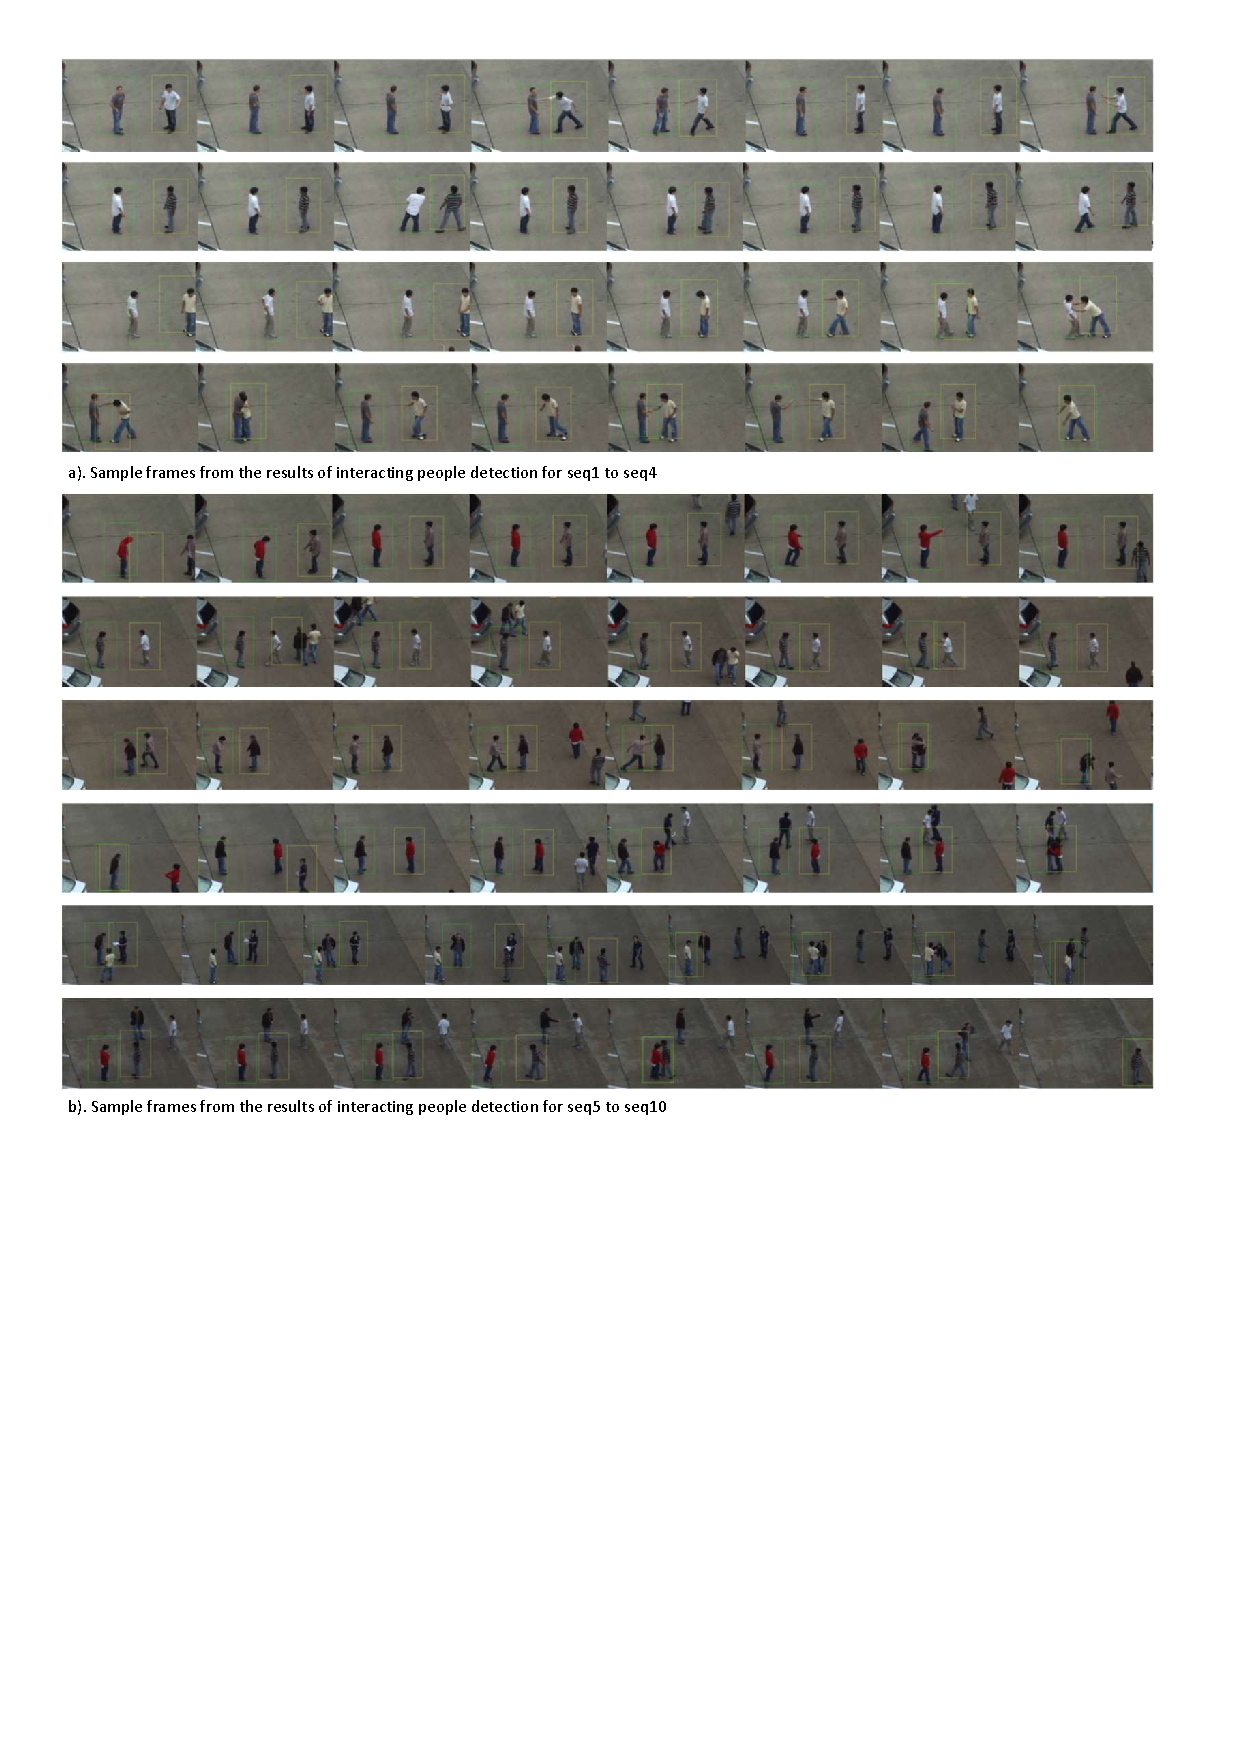
\includegraphics[trim=2cm 9cm 0cm 1cm]{fig01/interacting_person_det.pdf}
	\caption{Sample frames of the results of the spatial interacting people detection. The ground truth and detections are marked in green and red bounding boxes, respectively.}
	\label{fig:int_det}
\end{figure}

\begin{table}
	\caption{The average spatial overlap ratios of the bounding boxes between the detections and the ground truth for each video, evaluated on UT-Interaction set1.}
	\begin{center}
		\begin{tabular}{| m{2.5cm} || m{0.8cm} | m{0.8cm} | m{0.8cm} | m{0.8cm} | m{0.8cm} | m{0.8cm} | m{0.8cm} | m{0.8cm} | m{0.8cm} | m{0.8cm} |}
			\hline
			Videos & seq1 & seq2 & seq3& seq4& seq5& seq6& seq7& seq8& seq9& seq10 \\ \hline \hline
			Mean overlap ratios & 0.72 & 0.68 & 0.64 & 0.67& 0.68& 0.68& 0.75& 0.70& 0& 0.70 \\ \hline 
		\end{tabular}
		\label{table:mean_overlap_ratio}
	\end{center}
\end{table}
 
\subsection{Results of the interaction detection}
\subsubsection*{Experimental scheme}
Because the classification accuracy of the \(singleNet\_4096\) is slightly better than that of the \(fullNet\_2048\), we choose the trained \(singleNet\_4096\) as the interaction classifier for the interaction detection task. The 7-class \(singleNet\_4096\) interaction classifier is trained on the UT-Interaction dataset set1 from scratch with parameters listed in the Table \ref{table:network_settings}. 
\par
Since we already have the spatial locations of the interacting people after the process of the interacting people detection. We only need to slide a 3D window to generate candidate video clips. The value of 3D window depth \(l\) and sliding stride \(s\) are set to 48 and 8 respectively, see Section \ref{genIBB}. We perform the interaction detection on the 10 unsegmented videos of the UT-Interaction dataset set1, see Section \ref{ut-interaction}. 


\subsubsection*{Experimental results}
The experimental results of the interaction detection are illustrated in Figure \ref{fig:plot_temp} which shows the temporal overlaps between the interaction detections and the ground truth. The horizontal frame-axis is the time dimension (frames), and the vertical sequences-axis is the video sequences (10 for total). The time durations of the ground truth are annotated with green lines and their interaction class labels are annotated with green text above the corresponding lines.  And the time durations and interaction class labels of the detections are annotated with red lines and texts, respectively.

\begin{figure}
	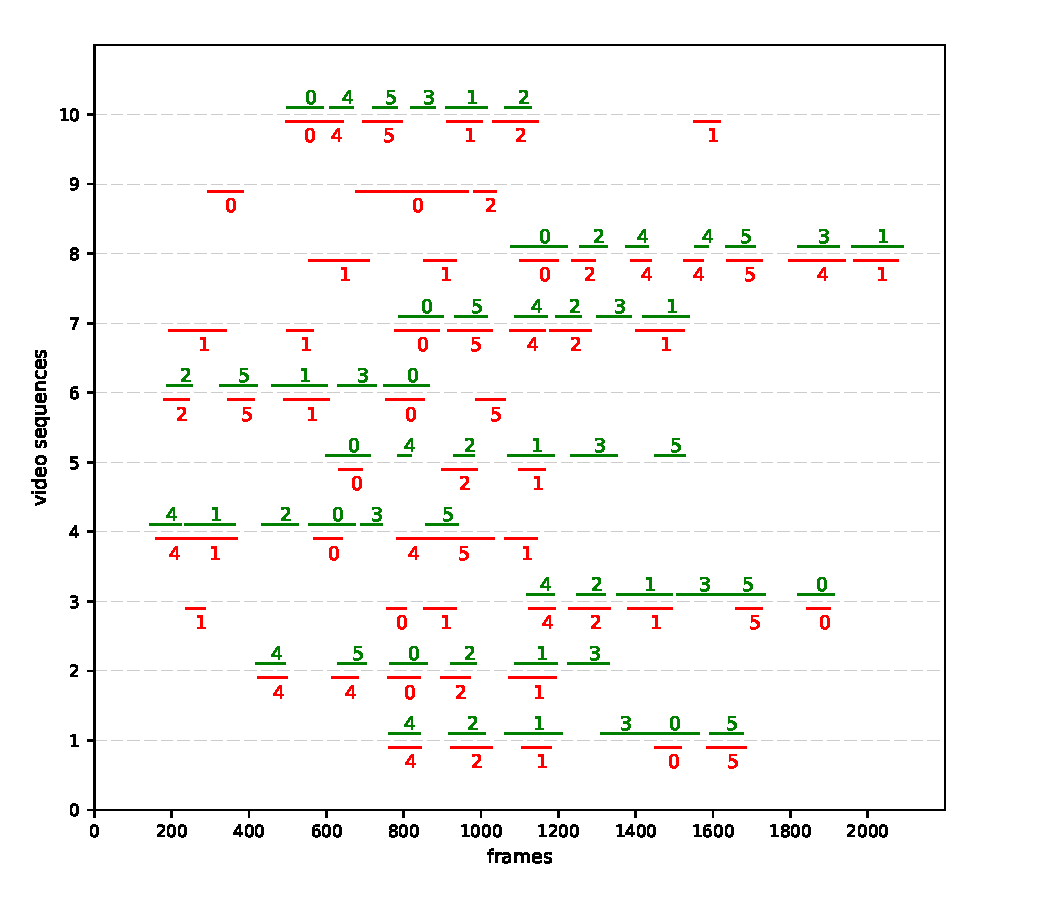
\includegraphics[trim=0.8cm 0cm 5cm 0cm]{fig01/plot_temp.pdf}
	\caption{The temporal overlaps between the interaction detections and the ground truth, evaluated on the 10 unsegmented videos of the UT-Interaction dataset set1. Ground truth data are marked in green, and the detections are marked in red.}
	\label{fig:plot_temp}
\end{figure}
\par

According to the results, there is no interaction with class label 
"3" ("Pointing") correctly detected by our interaction detector. This is because that we always draw our interacting bounding boxes over two interacting people, while only the location of the main actor was annotated in the ground truth, which is illustrated in Figure \ref{fig:label3}. We also failed to detect any interaction in the video sequence 9 since we have already failed to spatially detect the interacting people in this video. The precision and recall of the interaction detection under the configuration \(l = 48, s = 8\) evaluated on the 10 video sequences of the UT-Interaction set1 are illustrated in Table \ref{table:pr}. The intersection over union (IOU) between a detection and the ground truth is required to be larger than 0.5 according to the requirement of the dataset, see Section \ref{ut-interaction}. So, the overall precision and recall of our interaction detection evaluated on these 10 video sequences are 0.4 and 0.42, respectively. While if we lower the IOU threshold to 0.3, the overall precision and recall can be 0.67 and 0.63, respectively. The precision and recall score without consideration of class "Pointing" is illustrated in Table \ref{table:pr_ex3}. And the F1 scores over the different IOU thresholds are illustrated in Figure \ref{fig:plot_f1score}. Where F1 score is defined as following:
\begin{equation}
	F1\ socre = 2 \times \frac{precision \times recall}{precision + recall}
\end{equation}

\begin{figure}
	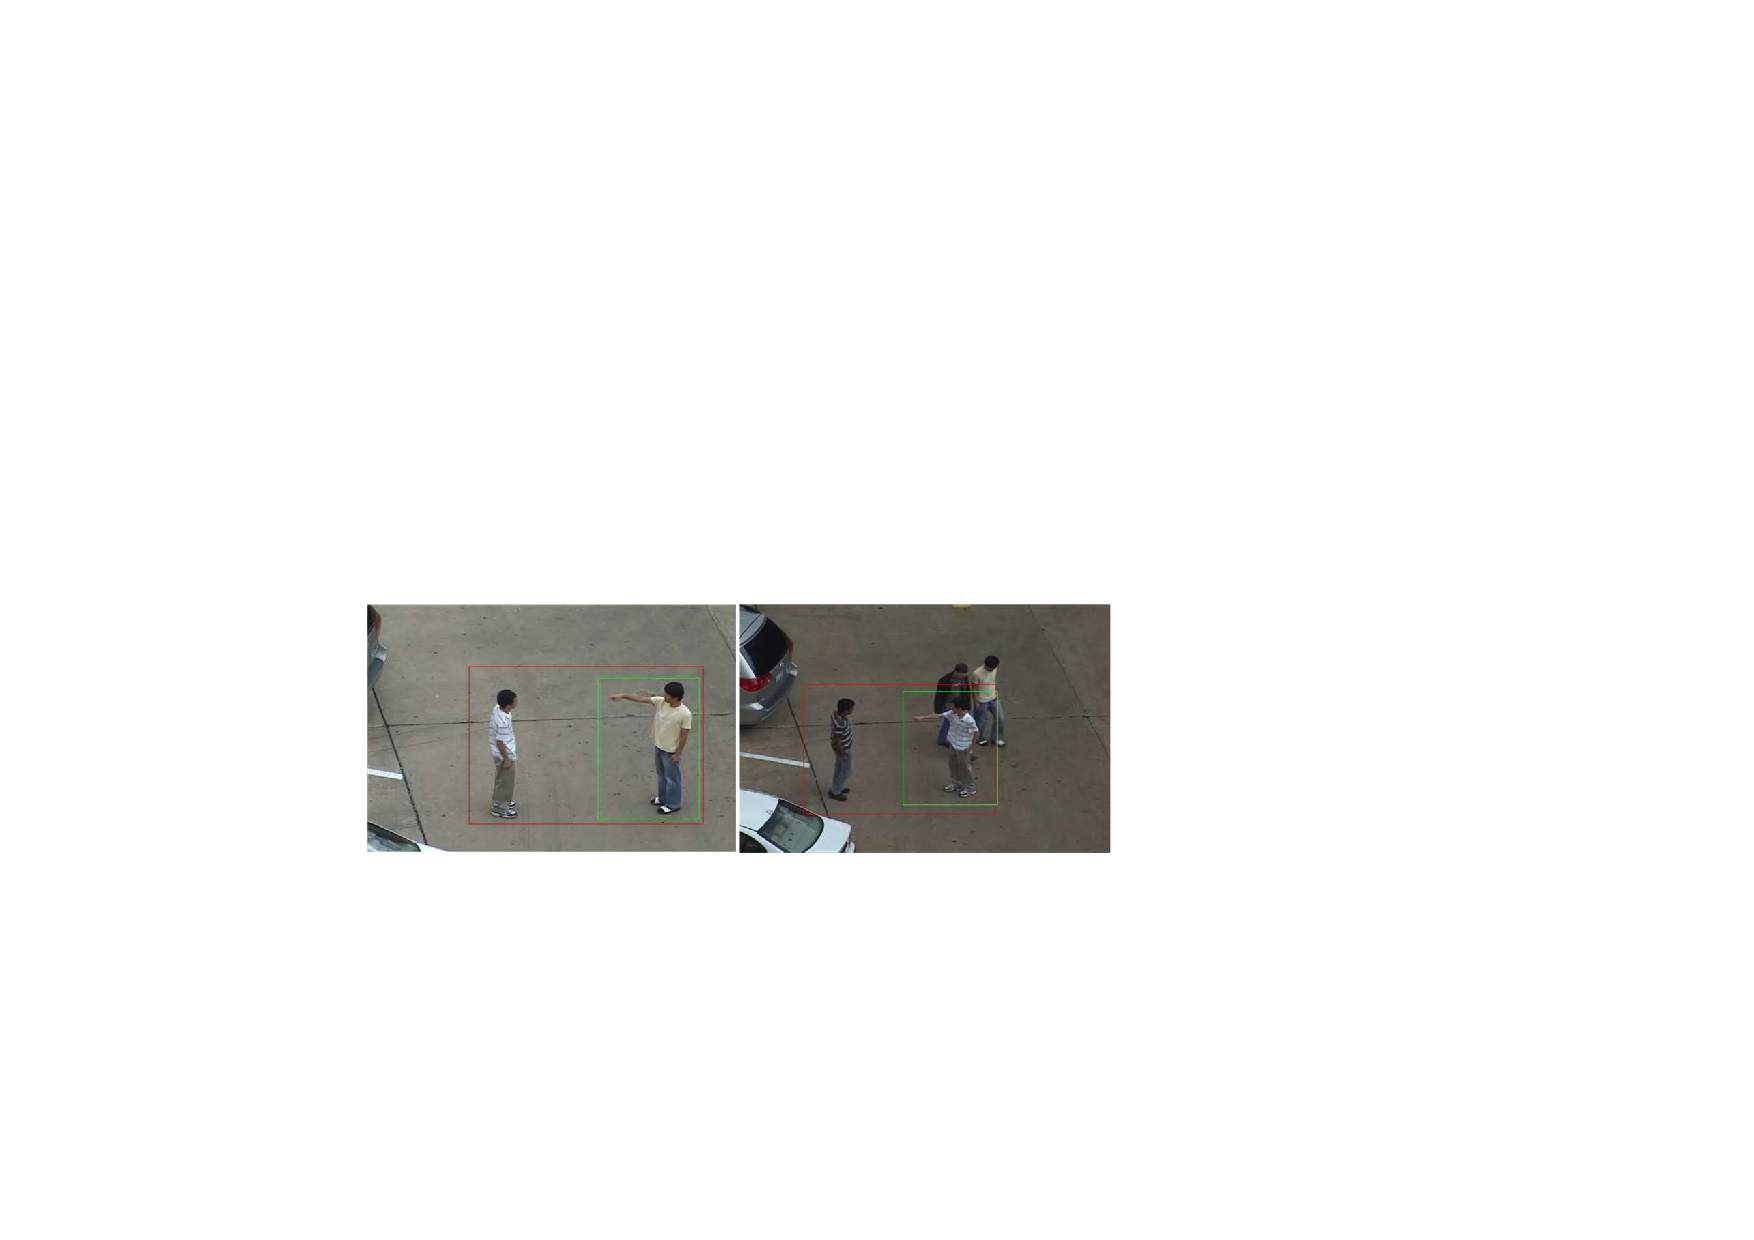
\includegraphics[trim=5cm 6cm 0cm 10cm]{fig01/label3.pdf}
	\caption{Spatial detection of interacting people. The green bounding boxes are the ground truth, while the reds are the detection results.  For the interactions with class label "3" ("Pointing"), only one person is annotated in the ground truth, while both interacting people are annotated by our detector. }
	\label{fig:label3}
\end{figure}
\par

\begin{table}
	\caption{The precision and recall of the interaction detection over the 10 video sequences of the UT-Interaction dataset set1, detector configuration (\(l=48, s=8\)).}
	\begin{center}
		\begin{tabular}{| m{2cm} || m{1.5cm} | m{1.5cm} | m{1.5cm} | m{1.5cm} | m{1.5cm} | m{1.5cm} |}
			\hline
			\multirow{2}{*}{Videos} & \multicolumn{2}{c|}{overlapRatio > 0.1} & \multicolumn{2}{c|}{overlapRatio>0.3} & \multicolumn{2}{c|}{\textbf{overlapRatio>0.5}} \\ \cline{2-7}
			 & precision & recall & precision & recall & precision & recall \\ \hline \hline
			 
			 seq1 & 1.0   & 0.83  & 1.0   & 0.83 & 0.6  & 0.5 \\ \hline
			 seq2 & 0.8   & 0.67  & 0.8   & 0.67 & 0.6  & 0.5 \\ \hline
			 seq3 & 0.63  & 0.83  & 0.5   & 0.67 & 0.5  & 0.67 \\ \hline
			 seq4 & 0.67  & 0.67  & 0.67  & 0.67 & 0.33 & 0.33 \\ \hline
			 seq5 & 1.0   & 0.5   & 1.0   & 0.5  & 0    &  0   \\ \hline
			 seq6 & 0.8   & 0.8   & 0.8   & 0.8  & 0.6  & 0.6  \\ \hline
			 seq7 & 0.71  & 0.83  & 0.71  & 0.83 & 0.57 & 0.67 \\ \hline
			 seq8 & 0.56  & 0.71  & 0.56  & 0.71 & 0.44 & 0.57 \\ \hline
			 seq9 & 0.17  & 0.17  & 0     & 0    & 0    & 0    \\ \hline
			 seq10 & 0.83 & 0.83  & 0.67  & 0.67 & 0.33 & 0.33 \\ \hline
			 overall & 0.72 & 0.68 & 0.67 & 0.63 & 0.4  & 0.42 \\ \hline	 
		\end{tabular}
		\label{table:pr}
	\end{center}
\end{table}


\begin{table}
	\caption{The precision and recall of the interaction detection over the 10 video sequences of the UT-Interaction dataset set1 without class "Pointing", detector configuration (\(l=48, s=8\)).}
	\begin{center}
		\begin{tabular}{| m{2cm} || m{1.5cm} | m{1.5cm} | m{1.5cm} | m{1.5cm} | m{1.5cm} | m{1.5cm} |}
			\hline
			\multirow{2}{*}{Videos} & \multicolumn{2}{c|}{overlapRatio > 0.1} & \multicolumn{2}{c|}{overlapRatio>0.3} & \multicolumn{2}{c|}{\textbf{overlapRatio>0.5}} \\ \cline{2-7}
			& precision & recall & precision & recall & precision & recall \\ \hline \hline
			
			seq1 & 1.0   & 1.0   & 1.0   & 1.0  & 0.6  & 0.6 \\ \hline
			seq2 & 0.8   & 0.8   & 0.8   & 0.8  & 0.6  & 0.6 \\ \hline
			seq3 & 0.63  & 1.0   & 0.5   & 0.8  & 0.5  & 0.8 \\ \hline
			seq4 & 0.67  & 0.8   & 0.67  & 0.8  & 0.33 & 0.4 \\ \hline
			seq5 & 1.0   & 0.6   & 1.0   & 0.6  & 0    &  0   \\ \hline
			seq6 & 0.8   & 1.0   & 0.8   & 1.0  & 0.6  & 0.75  \\ \hline
			seq7 & 0.71  & 1.0   & 0.71  & 1.0  & 0.57 & 0.8 \\ \hline
			seq8 & 0.56  & 0.83  & 0.56  & 0.83 & 0.44 & 0.6 \\ \hline
			seq9 & 0.17  & 0.2   & 0     & 0    & 0    & 0    \\ \hline
			seq10 & 0.83 & 0.1.0  & 0.67  & 0.8  & 0.33 & 0.4 \\ \hline
			overall & 0.72 & 0.82 & 0.67 & 0.76 & 0.4  & 0.5 \\ \hline	 
		\end{tabular}
		\label{table:pr_ex3}
	\end{center}
\end{table}

\begin{figure}
	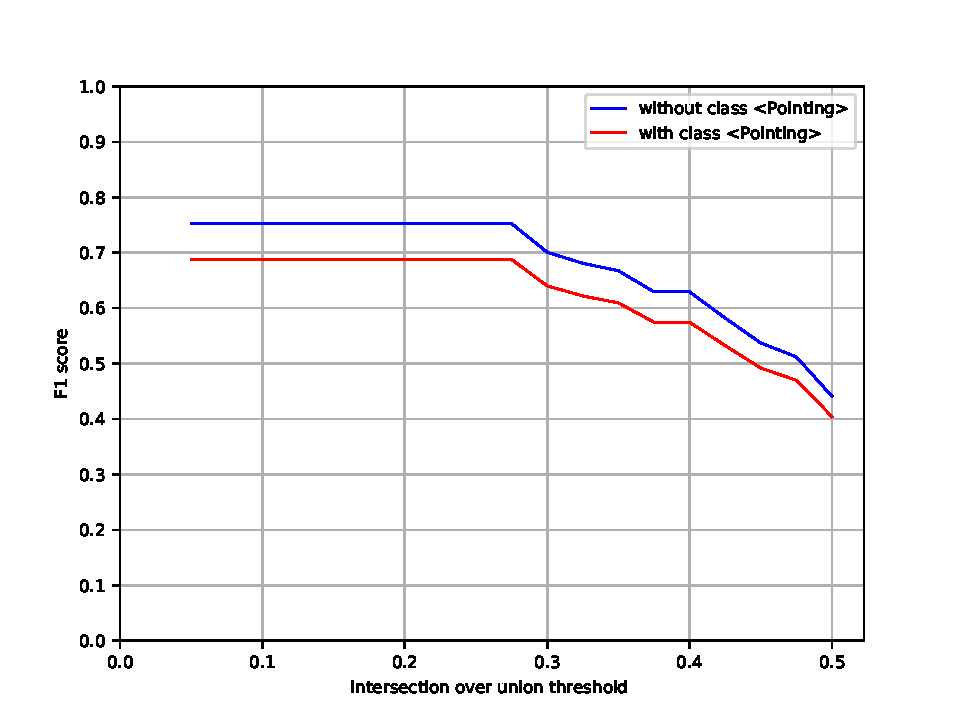
\includegraphics[trim=0cm 0cm 0cm 0cm]{fig01/plot_f1score.pdf}
	\caption{The F1 score over different IOU threshold.}
	\label{fig:plot_f1score}
\end{figure}
\par

%=========================================================